\chapter[The Fermilab Muon $g-2$ experiment]{The Fermilab Muon $g-2$\\ experiment}\label{chap:3}

The Muon $g-2$ experiment at Fermilab (E989) is the latest iteration of a six decade-long campaign to both measure the muon magnetic anomaly, $a_{\mu}$, and search for the muon EDM. E989 builds on the foundations laid by early efforts the Columbia-Nevis and University of Liverpool cyclotrons in the late 1950s, through a trio of direct measurements at \textit{European Organisation for Nuclear Research} (CERN) from the early 1960s to late 1970s, to the BNL E821 experiment in the 1990s and early 2000s -- even reusing the superconducting magnetic storage ring from E821 \cite[and references therein]{LeeHistory}. This most recent experiment makes use of the intense muon beam available from Fermilab's powerful accelerators, as well upgraded instrumentation, to target an unprecedented precision of 140 ppb on $a_{\mu}$, and a world-leading muon EDM upper limit of $\sim10^{-21}$ $e\cdot$cm \cite{TDR}. This chapter will outline the specific experimental techniques and hardware that comprise the E989 experiment.

\section{Overview}

E989 is designed to receive a beam of relativistic, longitudinally polarised muons and hold them in a stable circular orbit through a vertically aligned, homogeneous magnetic field. Following a time-dilated lifetime of \SI{64.4}{\micro\second}, the muons decay, and their much less massive decay products (positrons) curl away from the storage region, towards to centre of the ring. The decay positrons carry with them information pertaining to both $a_{\mu}$ and the muon EDM, which is measured by a suite of detectors instrumenting the ring interior. The magnetic field is precisely measured by a system of NMR probes. A photograph of the experiment is shown in Figure \ref{fig:E989_photo}. A schematic diagram of the experiment may be found on the final page of this chapter, in Figure \ref{fig:RingSchematic}.

\begin{figure}[t!]
\centering{}
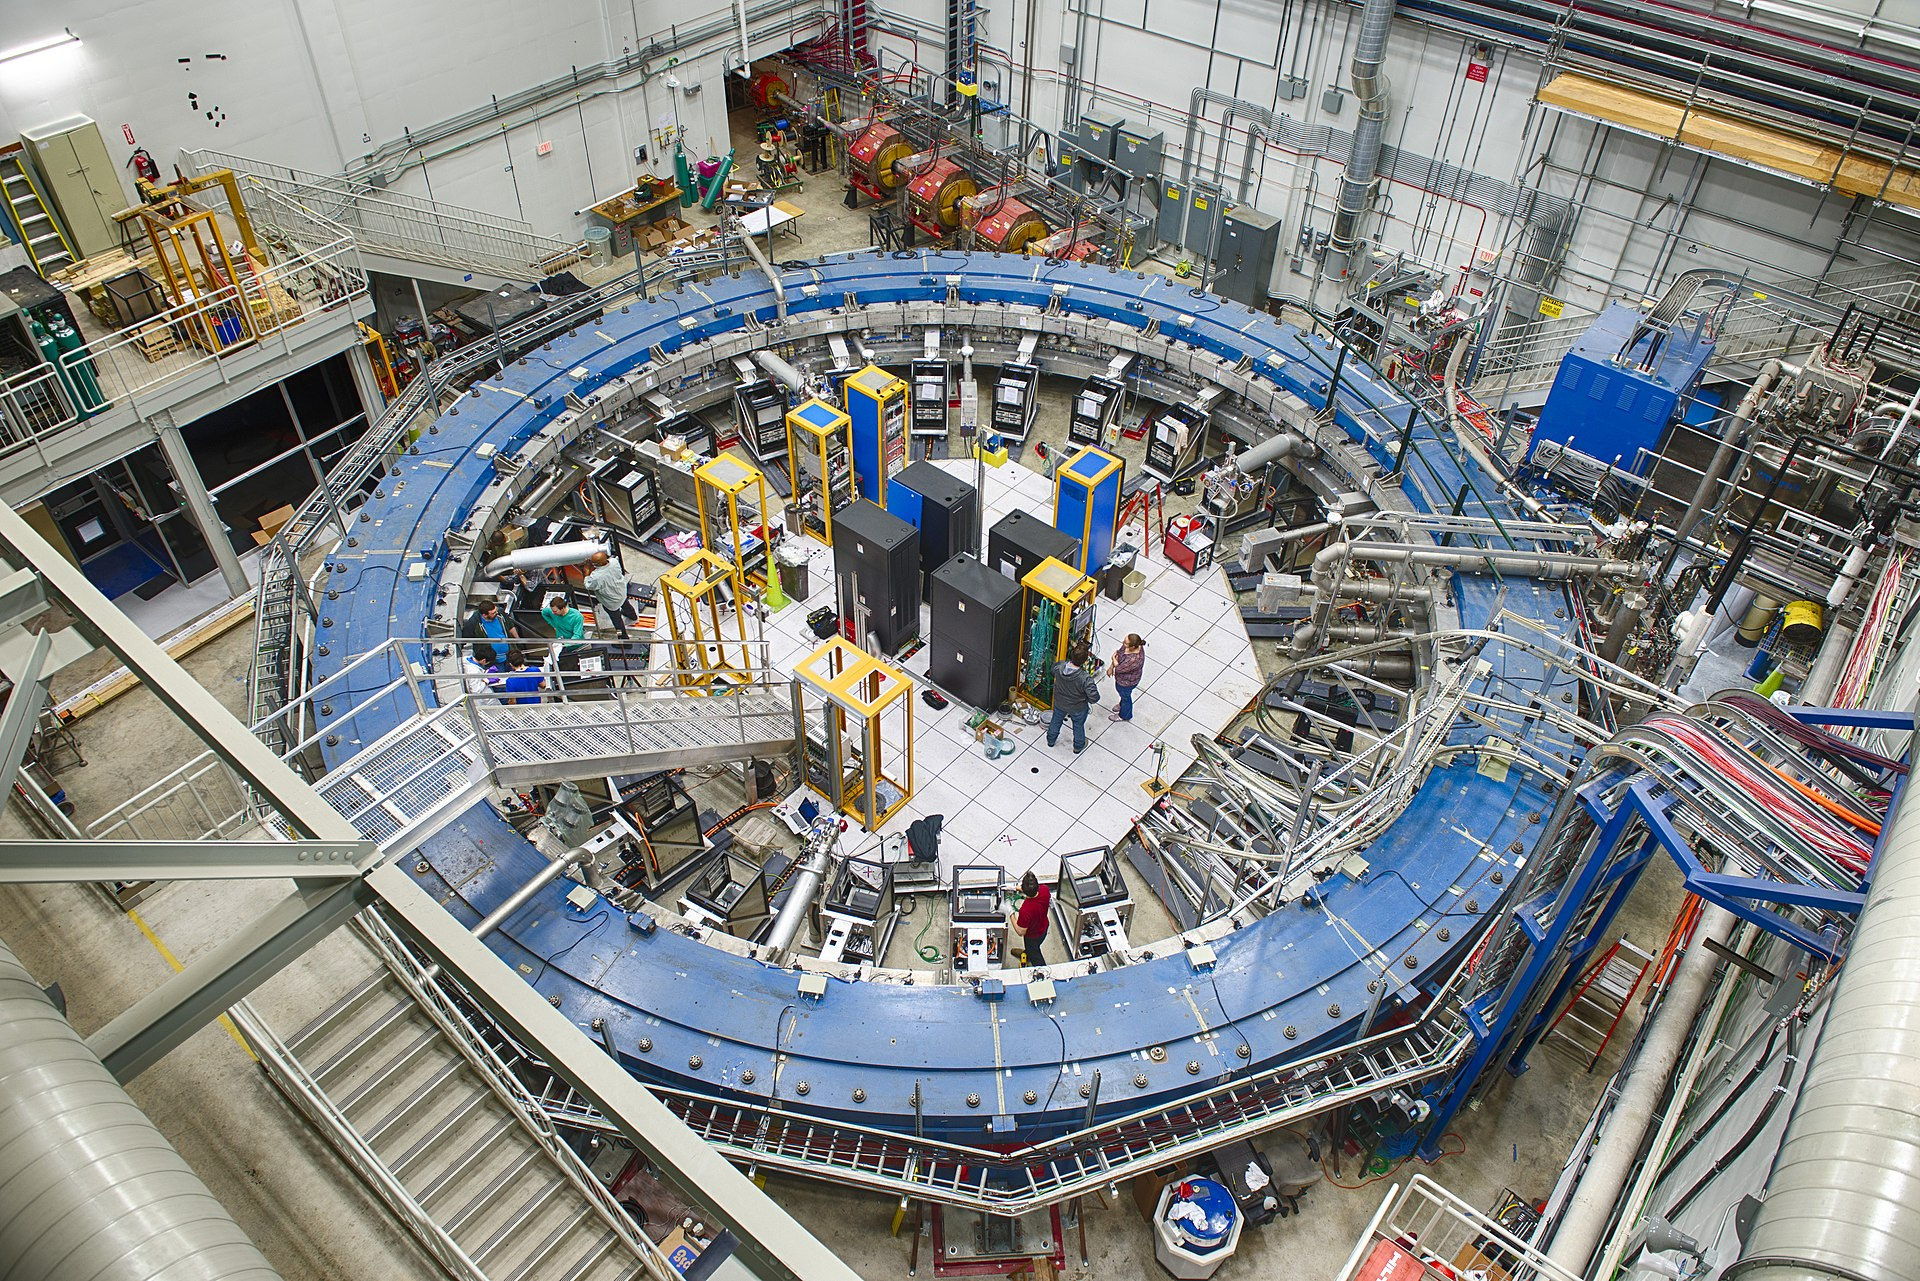
\includegraphics[trim={0 0 0 0},clip,width=.89\textwidth]{Images/Chapter3/E989_photo.jpg}
\caption{A photograph of the Fermilab Muon $g-2$ experiment (E989).}
\label{fig:E989_photo}
\end{figure}
%
%
\section{Muon production}

\begin{figure}[t!]
\centering{}
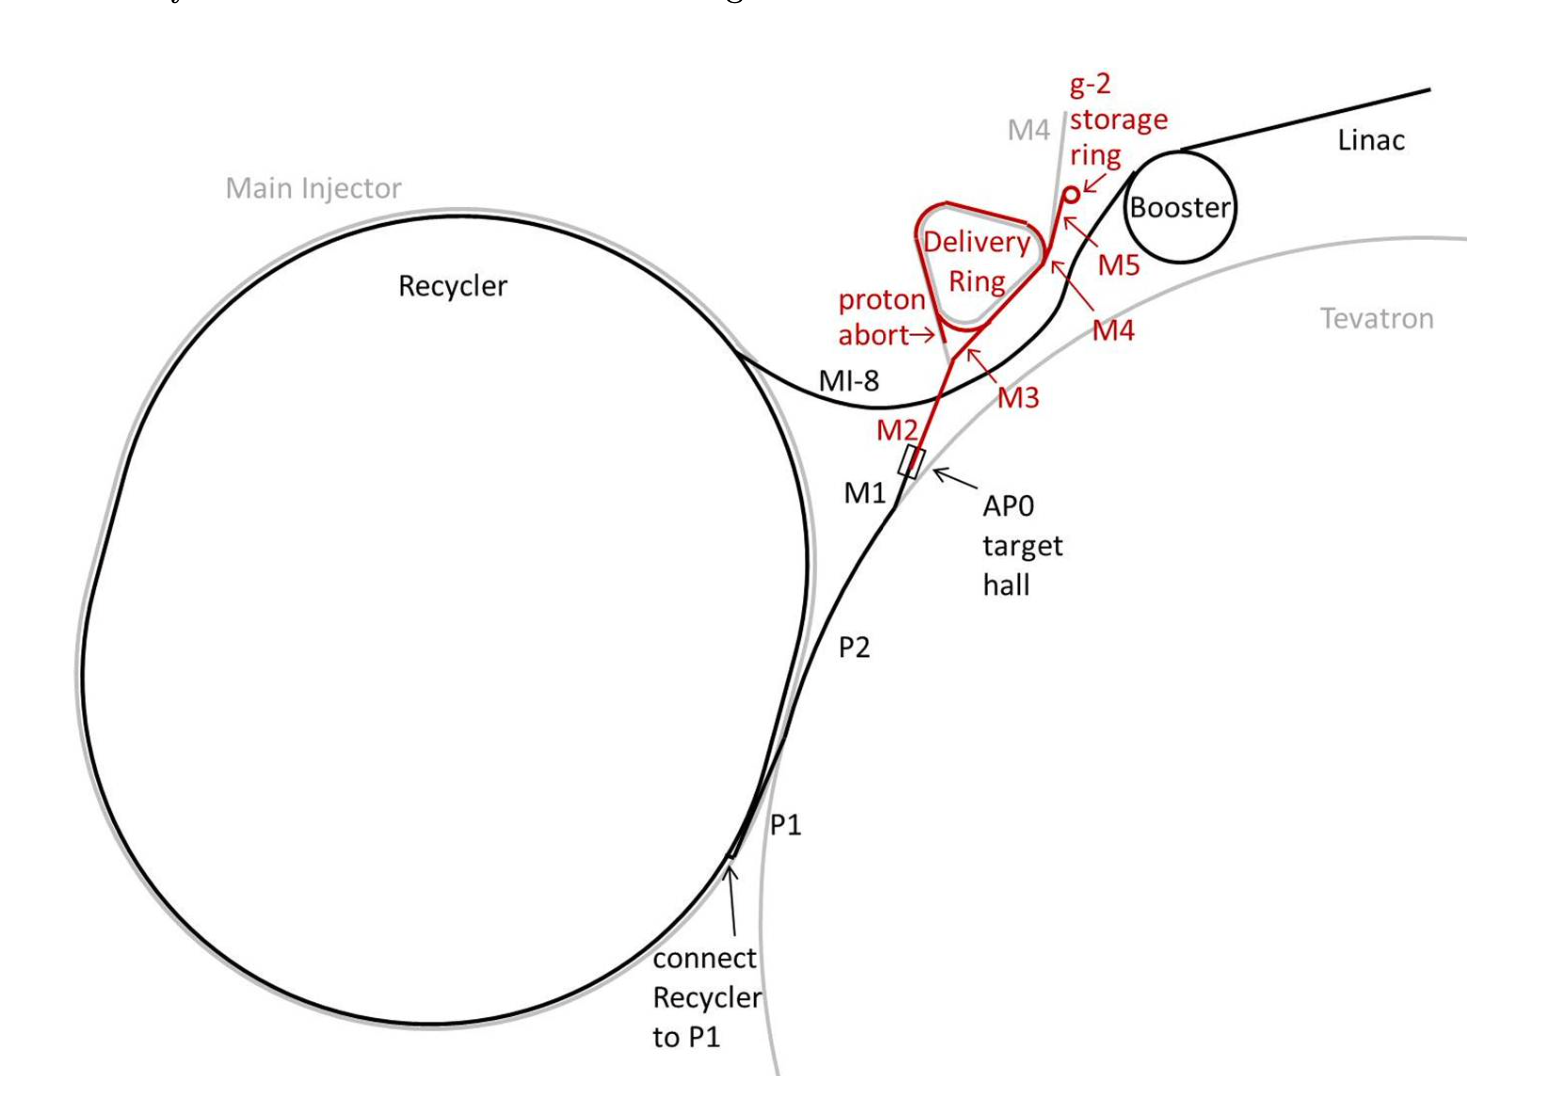
\includegraphics[trim={0 0 0 0},clip,width=.89\textwidth]{Images/Chapter3/AcceleratorComplex.png}
\caption{A schematic of the Fermilab accelerator complex, which delivers an intense and highly spin polarised beam of 3.094 GeV positive muons to the E989 storage ring. Image reproduced from \cite{TDR}.}
\label{fig:AcceleratorComplex}
\end{figure}  

\begin{figure}[t!]
\centering{}
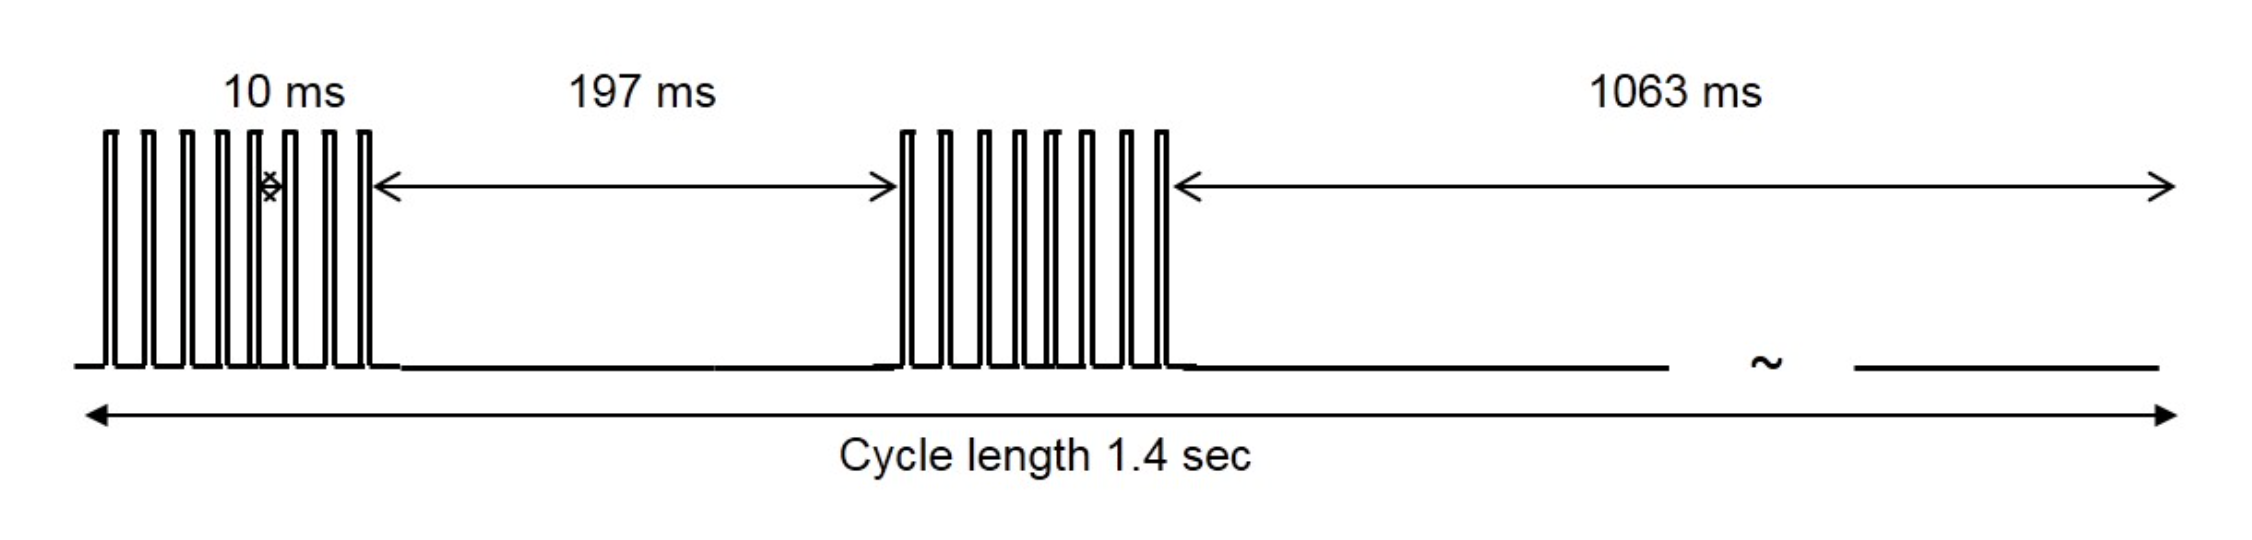
\includegraphics[trim={0 0 0 0},clip,width=.89\textwidth]{Images/Chapter3/TimingStructure.png}
\caption{The timing of beam pulses delivered to E989 over a single accelerator supercycle. Image reproduced from \cite{TDR}.}
\label{fig:TimingStructure}
\end{figure}

A large part of the motivation for conducting E989 at Fermilab was the availability of a highly intense muon beam from its vast accelerator complex, a schematic of which is show in Figure \ref{fig:AcceleratorComplex}. The beamline begins at the linear accelerator (linac), where hydrogen gas is ionised and accelerated, before being delivered as beam of protons to a synchrotron known as the `booster'. The booster accelerates the protons to 8 GeV and separates them into bunches of $4\times10^{12}$, which are then passed to a second synchrotron known as the `recycler'. The purpose of the recycler is to separate the intial bunches into four sets of $1\times10^{12}$, each with a width in time of \SI{120}{\nano\second}, which is less than the \SI{149.2}{\nano\second} cyclotron period of the E989 storage ring. This `re-bunching' process is undertaken with the requirements of E989 in mind, the aim being to bring the eventual rate of flux within the tolerances of the detectors and data acquisition system (DAQ). Following this, the \SI{120}{\nano\second} bunches are separated by time interval of at least \SI{10}{\milli\second} and delivered along the in groups of eight to the target hall. Over a full \SI{1.4}{\second} accelerator supercyle, E989 receives sixteen pulses at an average rate of \SI{11.4}{\hertz}, where the timing structure of proton delivery is illustrated in Figure \ref{fig:TimingStructure}. 

Once delivered to the target hall, the protons are directed at an Inconel target, a high-Z nickel-iron alloy, where the ensuing proton-nucleon interactions results in the production of large quantities of pions. The pions are focused by a lithium lens downstream of the production target, and a bending magnet is used to select positive pions with a momentum within $\pm10$\% of 3.11 GeV. The beam is then sent to the `delivery ring', where the pions that have not already decayed into muons are given time to do so by the process given in Equation \ref{eqn:PionDecay}. Within the delivery ring, muons with highest momentum are selected, ensuring that the muon beam is highly spin polarised in the manner shown in Figure \ref{fig:PionDecay}. The delivery ring also serves the purpose of removing residual protons and deuterons by use of an electromagnetic kicker. Finally, the muons are sent to the E989 experiment hall, where they pass through four electromagnetic focusing quadrupoles before being injected into the storage ring as a highly polarised beam with a momentum spread of $\pm1.6$\% \cite{BeamDynamics} about the magic momentum, 3.094 GeV. Further discussion on the accelerator complex and muon delivery to E989 may be found in \cite{FermilabBeamline}.

\section{Injection and storage}\label{sec:InjectionAndStorage}

\subsection{The inflector}

\begin{figure}[b!]
\centering{}
\subfloat[]{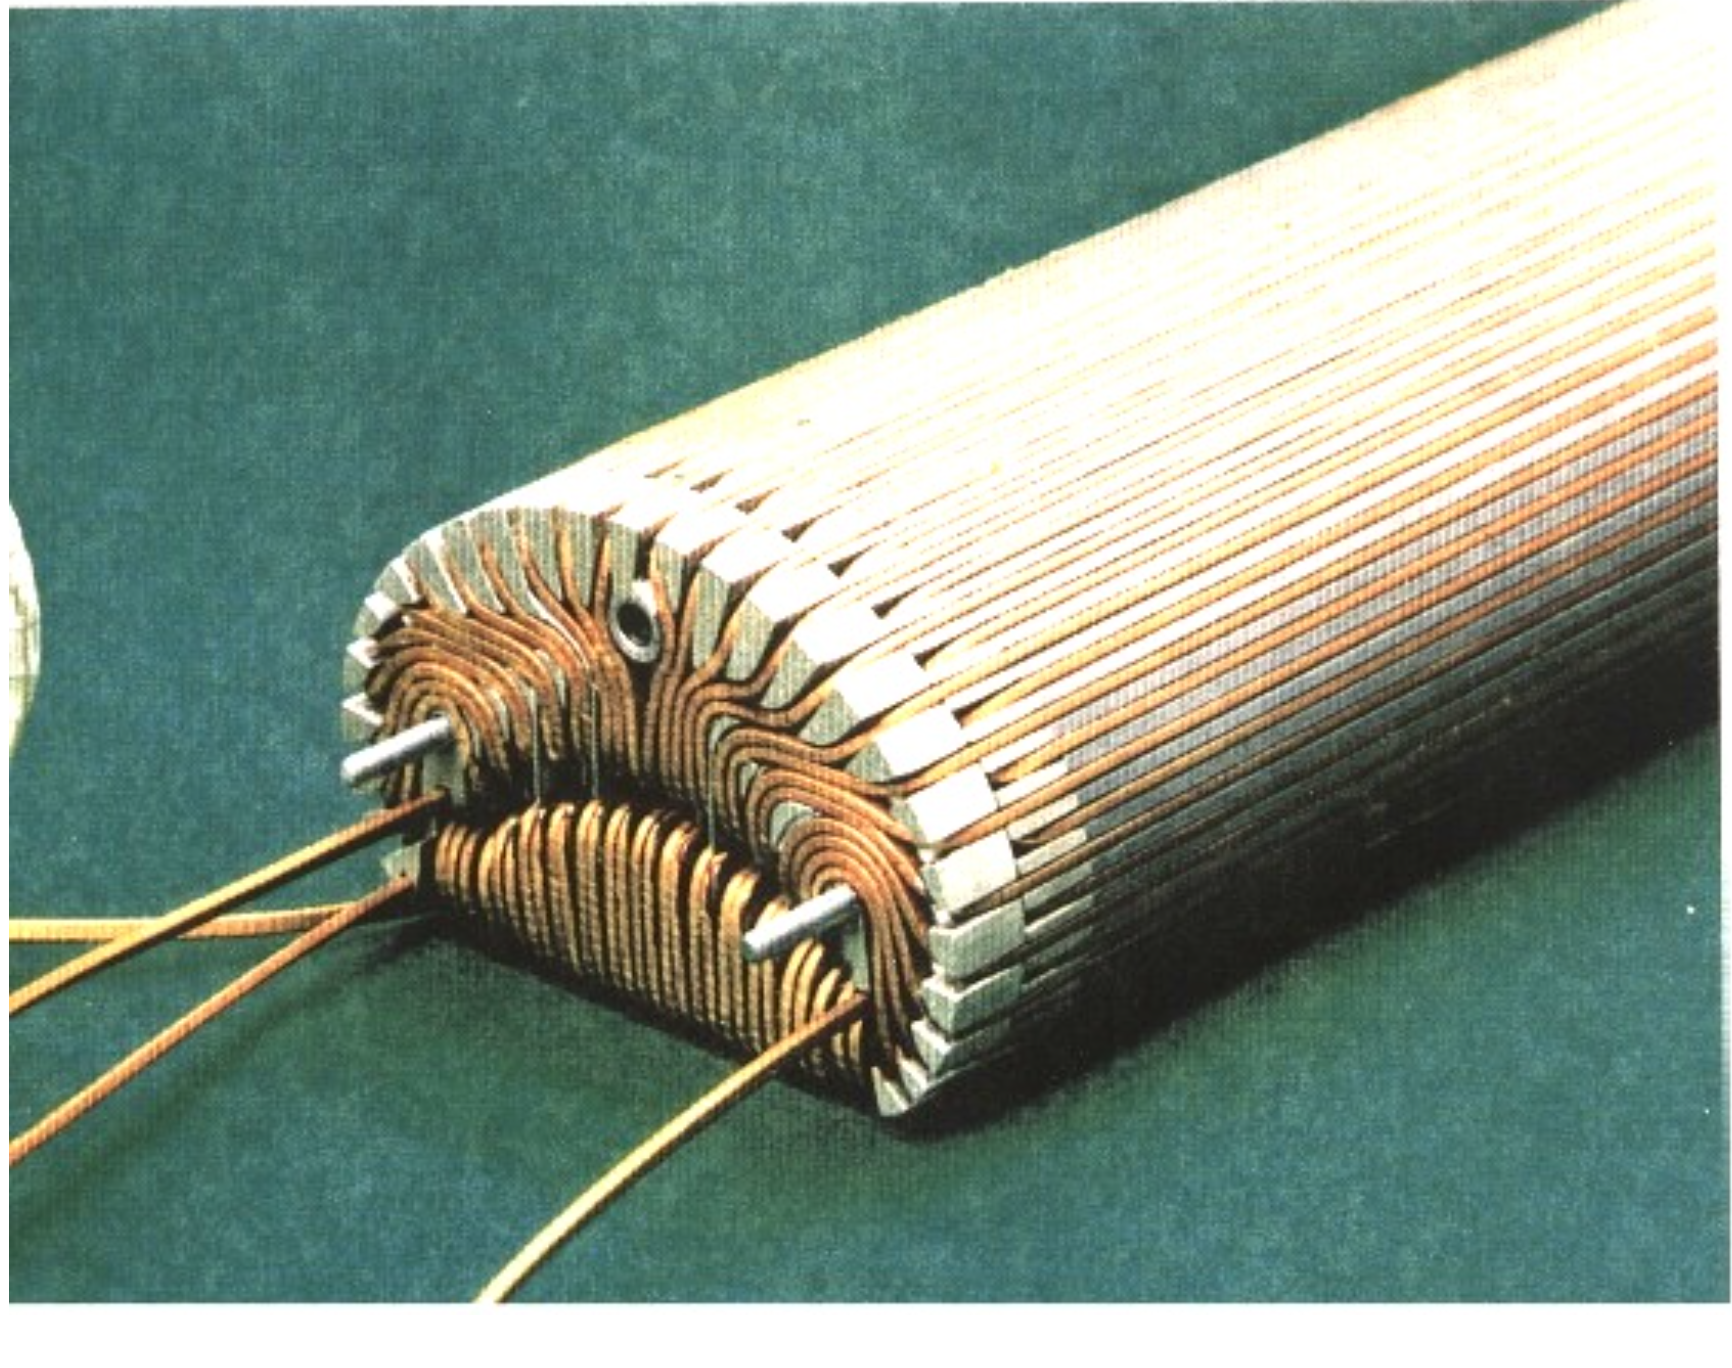
\includegraphics[trim={3 2 3 2},clip,width=.49\textwidth]{Images/Chapter3/InflectorPhoto.png}\label{subfig:InflectorPhoto}}
\hfill
\hfill
\subfloat[]{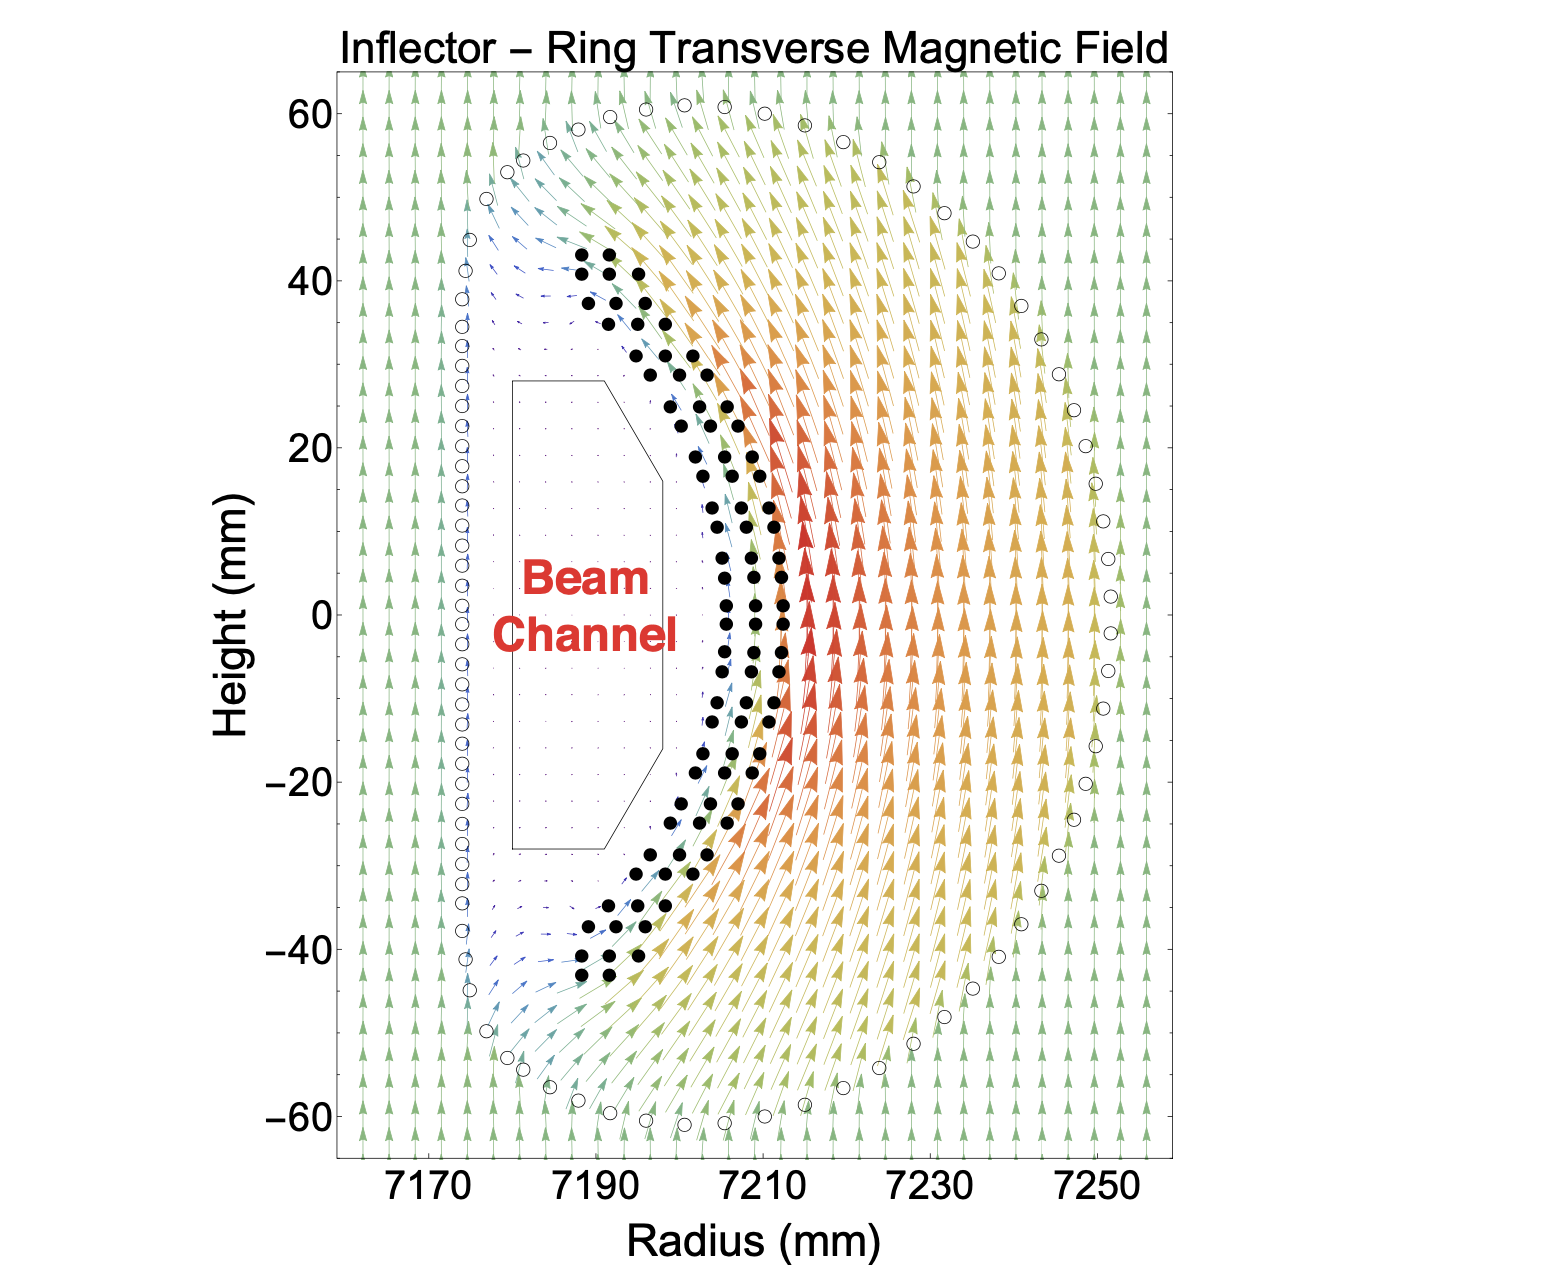
\includegraphics[trim={0 0 0 0},clip,width=.49\textwidth]{Images/Chapter3/InflectorField.png}\label{subfig:InflectorField}}
\caption{(a) A photograph showing an end view of the inflector; (b) the sum of the inflector and main magnet fields, showing the field free region through which the beam passes without being deflected. Images reproduced from \cite{InflectorCommissioning}.}
\label{fig:Inflector}
\end{figure} 

The E989 main magnet is designed to produce a homogenous magnetic field around the full azimuth of the ring, necessitating a monolithic construction with as few gaps as possible. Because of this, the muons must be injected directly through the magnet yoke (discussed in Section \ref{sec:Field}). In order to achieve this without the beam being deflected, the muons are passed through a specialised field cancelling device called the `superconducting inflector magnet', or `inflector', which is oriented at an approximate tangent to the storage ring. The inflector consists of superconducting niobium-titanium-copper-aluminium coils, wrapped to give the unique geometry of electric currents required to almost completely cancel the main magnetic field, shown in Figure \ref{fig:Inflector}. The positioning of the inflector relative to storage ring as whole is shown in Figure \ref{fig:RingSchematic}. The time at which the beam passes through the inflector marks the beginning of period known as a `fill'\footnote{The initial time of the fill, $t=0$, is defined by a detector called the `T0 counter' described in Section \ref{subsec:Aux}.}. Further information on the inflector can be found in \cite{InflectorCommissioning}.

\subsection{The kickers}

The interior volume of the ring through which the muons circulate, the `storage region', must be free from obstruction. Because of this, the inflector is displaced from the central radius of the storage region, $R_{0}=7112$ mm, by \SI{77}{\milli\metre}. Without intervention, the muons would propagate once around the ring and collide with the inflector. In order to set the beam on a stable orbit, a large radial force must be applied to the beam, a `kick'. To achieve this, three electromagnetic kickers positioned at 90{\degree} from the inflector, denoted by K1 through K3 in Figure \ref{fig:RingSchematic}, provide a pulsed magnetic field sufficient to compensate for the initial displacement, centring the beam on $R_{0}$. Each kicker consists of two 1.27 m long aluminium plates, which is non-ferric so as not to perturb the magnetic field, positioned inside the storage ring vacuum. They are designed to produce an integrated vertical magnetic field of approximately 1.1 kG-m for a period of 120 ns, covering the full time width of the injected bunch, which dies away before the muons re-enter the kicker aperture following a cyclotron period of \SI{149.2}{\nano\second}. 

The intensity of the kicker pulse with time is given by the black curve in Figure \ref{subfig:KickerPulse}, showing how the peak is contained within the cyclotron period, indicated by dashed blue lines. A photograph of a spare set of kicker plates is shown by Figure \ref{subfig:KickerPulse}. Detailed discussion on the kicker system can be found in \cite{KickerPaper}.

\begin{figure}[t!]
\centering{}

\subfloat[The kicker pulse.]{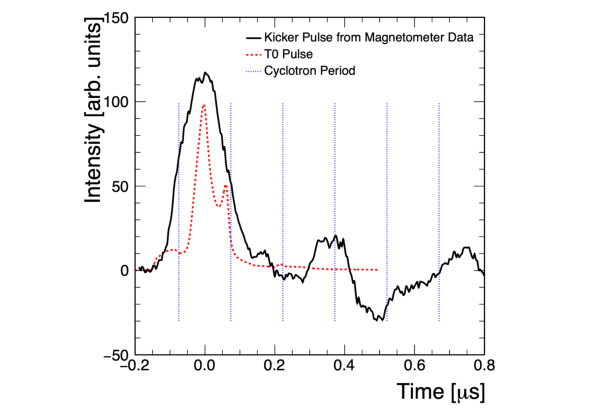
\includegraphics[trim={0 0 0 0},clip,width=.49\textwidth]{Images/Chapter3/KickerPulse_Wide2.pdf}\label{subfig:KickerPulse}}
\subfloat[Spare kicker plates.]{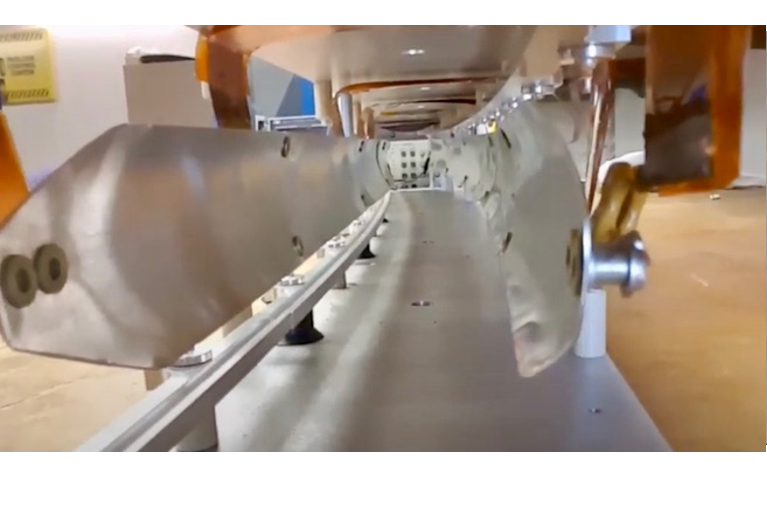
\includegraphics[trim={0 0 0 0},clip,width=.49\textwidth]{Images/Chapter3/SpareKickerPlates.pdf}\label{subfig:KickerPlates}}
\caption{(a) The intensity of the kicker pulse with time, shown by a black curve, where the \SI{120}{\nano\second} peak is contained within the \SI{149.2}{\nano\second} cyclotron period, indicated by dashed blue lines; (b) a photograph of a spare set of kicker plates. First image reproduced from \cite{BeamDynamics}, second image courtesy of A. P. Schreckenberger \cite{KickerPlates}.}
\label{fig:Kickers}
\end{figure} 


\subsection{The electrostatic quadrupoles}\label{sec:ESQs}


\begin{figure}[t!]
\centering{}
\subfloat[The ESQ field.]{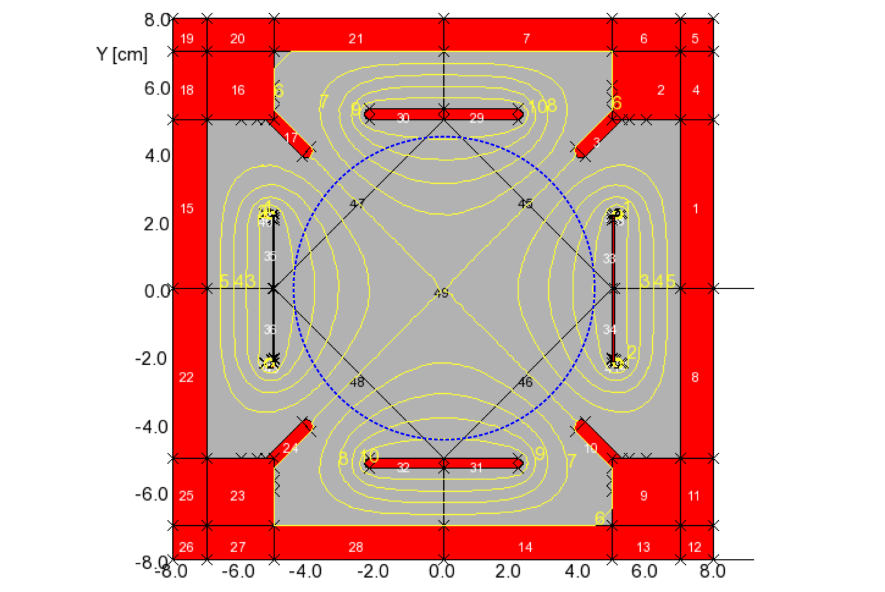
\includegraphics[trim={0 0 0 0},clip,width=.49\textwidth]{Images/Chapter3/QuadField.pdf}\label{subfig:QuadField}}
\subfloat[The ESQ plates.]{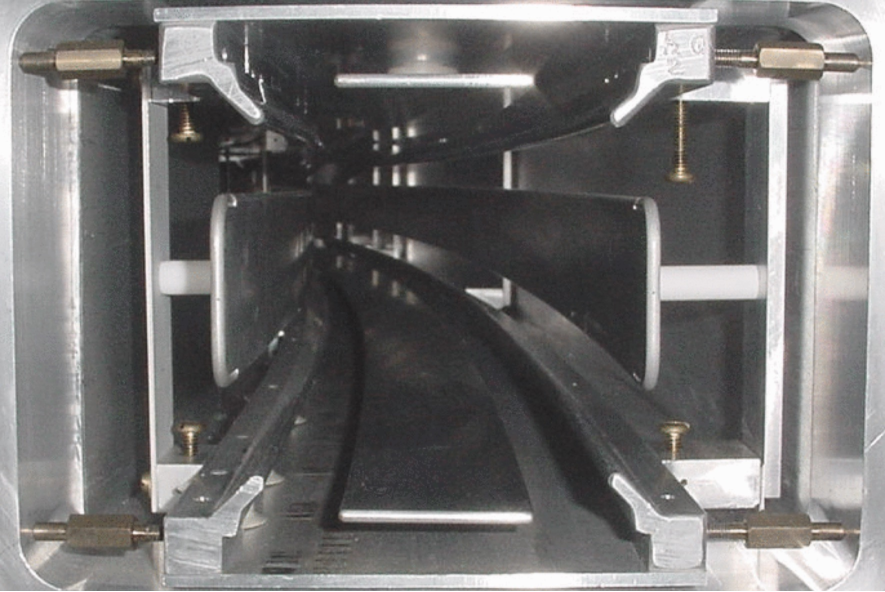
\includegraphics[trim={0 0 0 0},clip,width=.49\textwidth]{Images/Chapter3/QuadPlates.pdf}\label{subfig:QuadPlates}}
\caption{(a) A model of the ESQ field, where the yellow curves indicates lines of equal electrostatic potential; (b) a photograph of one set of ESQ plates, viewed from downstream. Images reproduced from \cite{TDR}.}
\label{fig:Quads}
\end{figure} 

In the ideal case, the kick would set the muons on a perfect orbit, whereby every muon is aligned with the tangent of circle defined by the ideal storage radius, and has an exclusively longitudinal component of momentum which is exactly equal to the magic momentum, $3.094$ GeV. In reality, the storage ring possesses a momentum acceptance of $\pm0.15$\% about this value \cite{BeamDynamics}, as previously noted in Chapter \ref{chap:2} Section \ref{sec:OmegaACorrections}, with momentum components in the radial and vertical directions. Because of this, the beam must be focused in order to prevent beam divergence and complete loss of storage after a few revolutions. The main dipole magnetic field focuses the beam radially\footnote{The ESQs have a defocusing effect along the radial axis, but combination of electric and magnetic fields is still adequate to provide net focusing.}, while vertical focusing is provided by four in-vacuum electrostatic quadrupoles (ESQs). The ESQs are spaced evenly around the ring, denoted by Q1 through Q4 in Figure \ref{fig:RingSchematic}, where they cover 43\% of the total azimuth --  leaving space for other in-vacuum storage ring components such as the inflector, kickers, and straw tracking detectors. A critical ESQ parameter is the field index, $n$, which relates the electric field gradient $\kappa = \partial E_{y} / \partial y$, to the strength of main magnetic dipole field, $B_{0}$, given by
%
\begin{equation}
  n = \frac{\kappa R_{0}}{v B_{0}} 
  \label{eqn:FieldIndex}
\end{equation}
%{}
where $R_{0}$ is the central radius of the storage region and $v$ is the muon velocity \cite{TDR}. %The above expression will be referenced again in Chapter 4. 

The ESQs also serve the important function of removing improperly stored muons, which are destined to exit the ring before decaying: contaminating the flux of decay positrons falling into the detectors. This process is known as `scraping', which begins at injection and lasts for \SI{7}{\micro\second}, after which the ESQs are ramped to their full set-point voltage \cite{BeamDynamics}. The scraping procedure involves charging the ESQ plates with asymmetric voltages to move the beam radially and vertically into five 45 mm radius copper collimators, which scatter muons on the tails of the beam distribution, causing them to lose energy and fall out of the storage region. After a total time of \SI{30}{\micro\second} after injection, the beam stabilises and the remaining muons are properly stored. Further information on the ESQs can be found in \cite{TDR}.

\section{Muon beam dynamics}\label{sec:BeamDynamics}

This section will describe the muon beam dynamics which are relevant to the work presented in this thesis. A more comphrensive review of beam dynamics at E989, as it applies to Run-1, may be found in \cite{BeamDynamics}.

\subsection{Coherent betatron oscillations}\label{subsec:CBO}

As discussed in Section \ref{sec:ESQs}, the combination of magnetic and electric fields in ring affect a restoring force on the muon beam in the vertical and radial directions, preventing divergence from the storage region. As a result, the beam undergoes simple harmonic motion in the radial and vertical directions, which may be described by the equations of motion 
%
\begin{equation}
  \frac{d^{2}x}{dt^{2}} = -\omega_{c}(1-n)\cdot x,
  \label{eqn:EOM_BOx}
\end{equation}
%
%
\begin{equation}
  \frac{d^{2}y}{dt^{2}} = -\omega_{c}n\cdot y,
  \label{eqn:EOM_BOy}
\end{equation}
%
where $\omega_{c}$ is the angular cyclotron frequency given by Equation \ref{eqn:Cyclotron}, and $n$ is the electric field index given by Equation \ref{eqn:FieldIndex}. In this context, this type of motion is referred to as `betatron oscillations'. The equations of motion may be solved by substitution of the oscillatory functions
%
\begin{equation}
  x(t) = A_{x}\cos(\omega_{x}t-\phi_{x}),
  \label{eqn:SLN_BOx}
\end{equation}
%
\begin{equation}
  y(t) = A_{y}\cos(\omega_{y}t-\phi_{y}),
  \label{eqn:SLN_BOy}
\end{equation}
%
giving the betatron frequencies of  

\begin{equation}
  f_{x} = f_{c}\cdot\sqrt{1-n},
  \label{eqn:omegaBOx}
\end{equation}
%
\begin{equation}
  f_{y} = f_{c}\cdot\sqrt{n},
  \label{eqn:omegaBOy}
\end{equation}
%
where $f = \omega/2\pi$. 

The  muons that comprise the beam share a common phase space distribution following injection and the kick, so that their individual betatron oscillations are coherent: causing the entire beam to move as one. This beam motion is termed `coherent betatron oscillations' (CBO), shown in Figure \ref{fig:CBO} as measured by the straw trackers described in Section \ref{subsec:Trackers}. 

\begin{figure}[t!]
\centering{}
\subfloat[Radial CBO.]{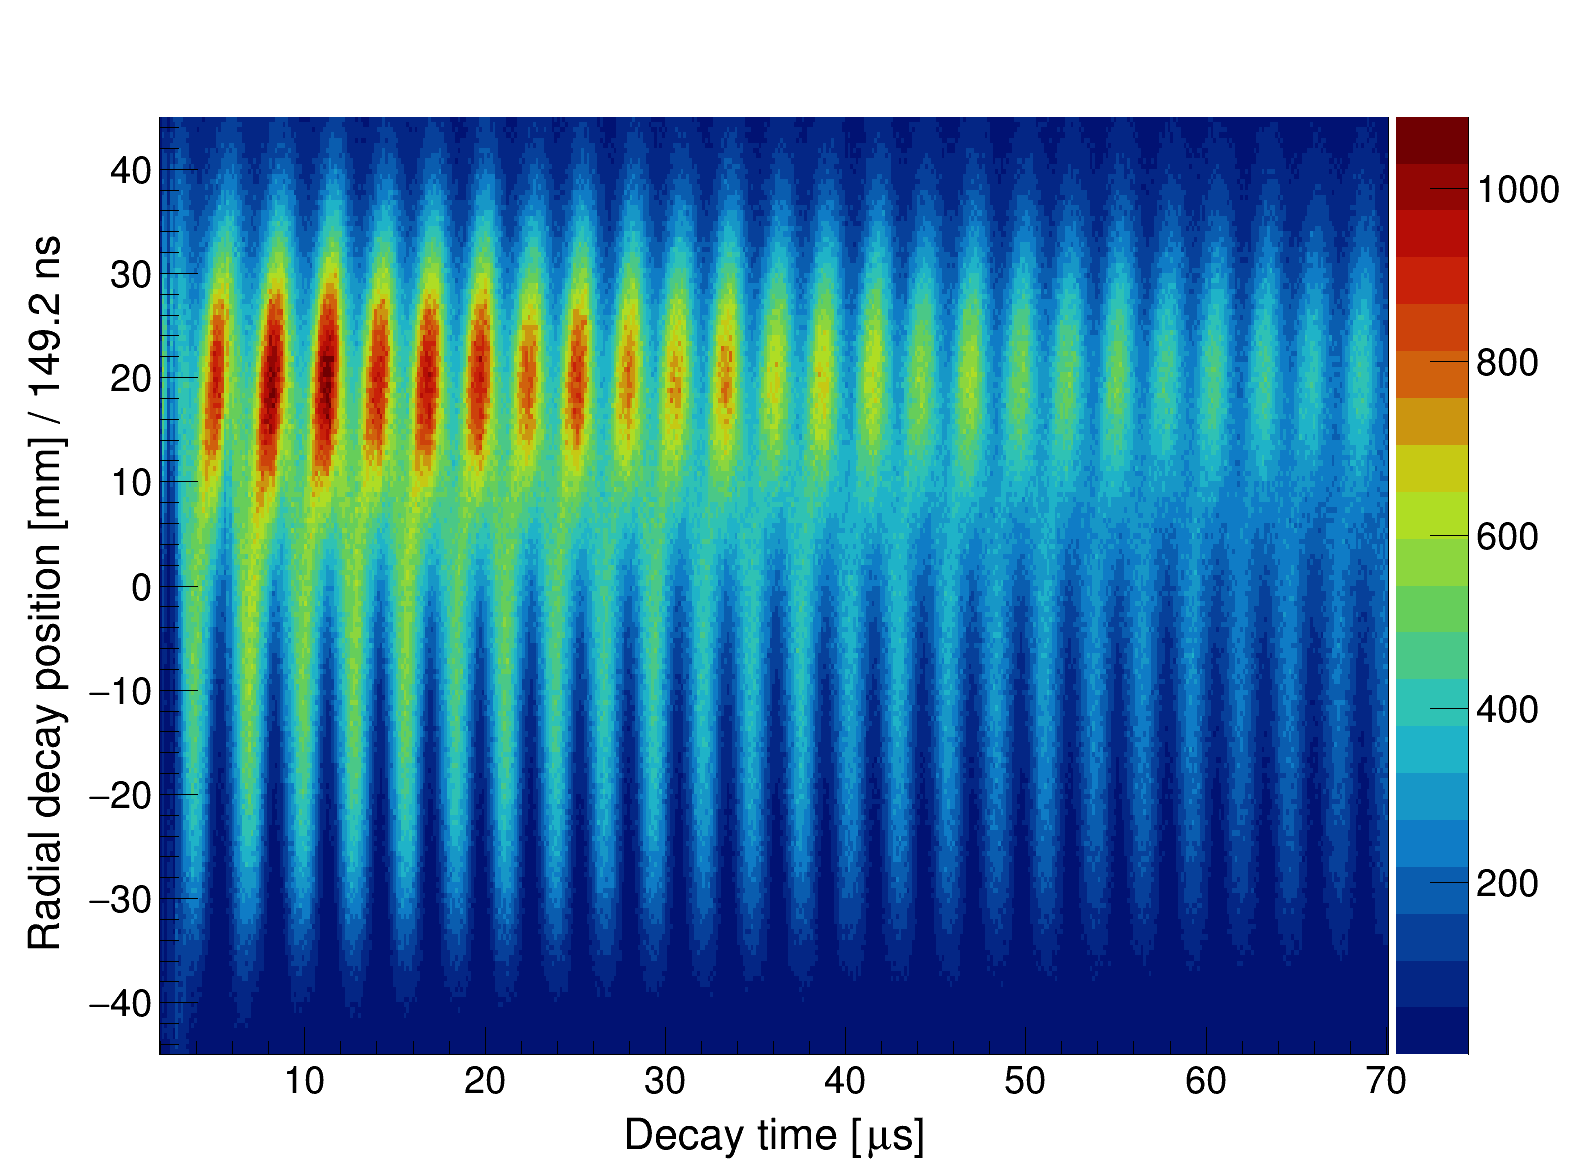
\includegraphics[trim={0 0 0 0},clip,width=.49\textwidth]{Images/Chapter3/R_vs_t.png}}
\subfloat[Vertical CBO.]{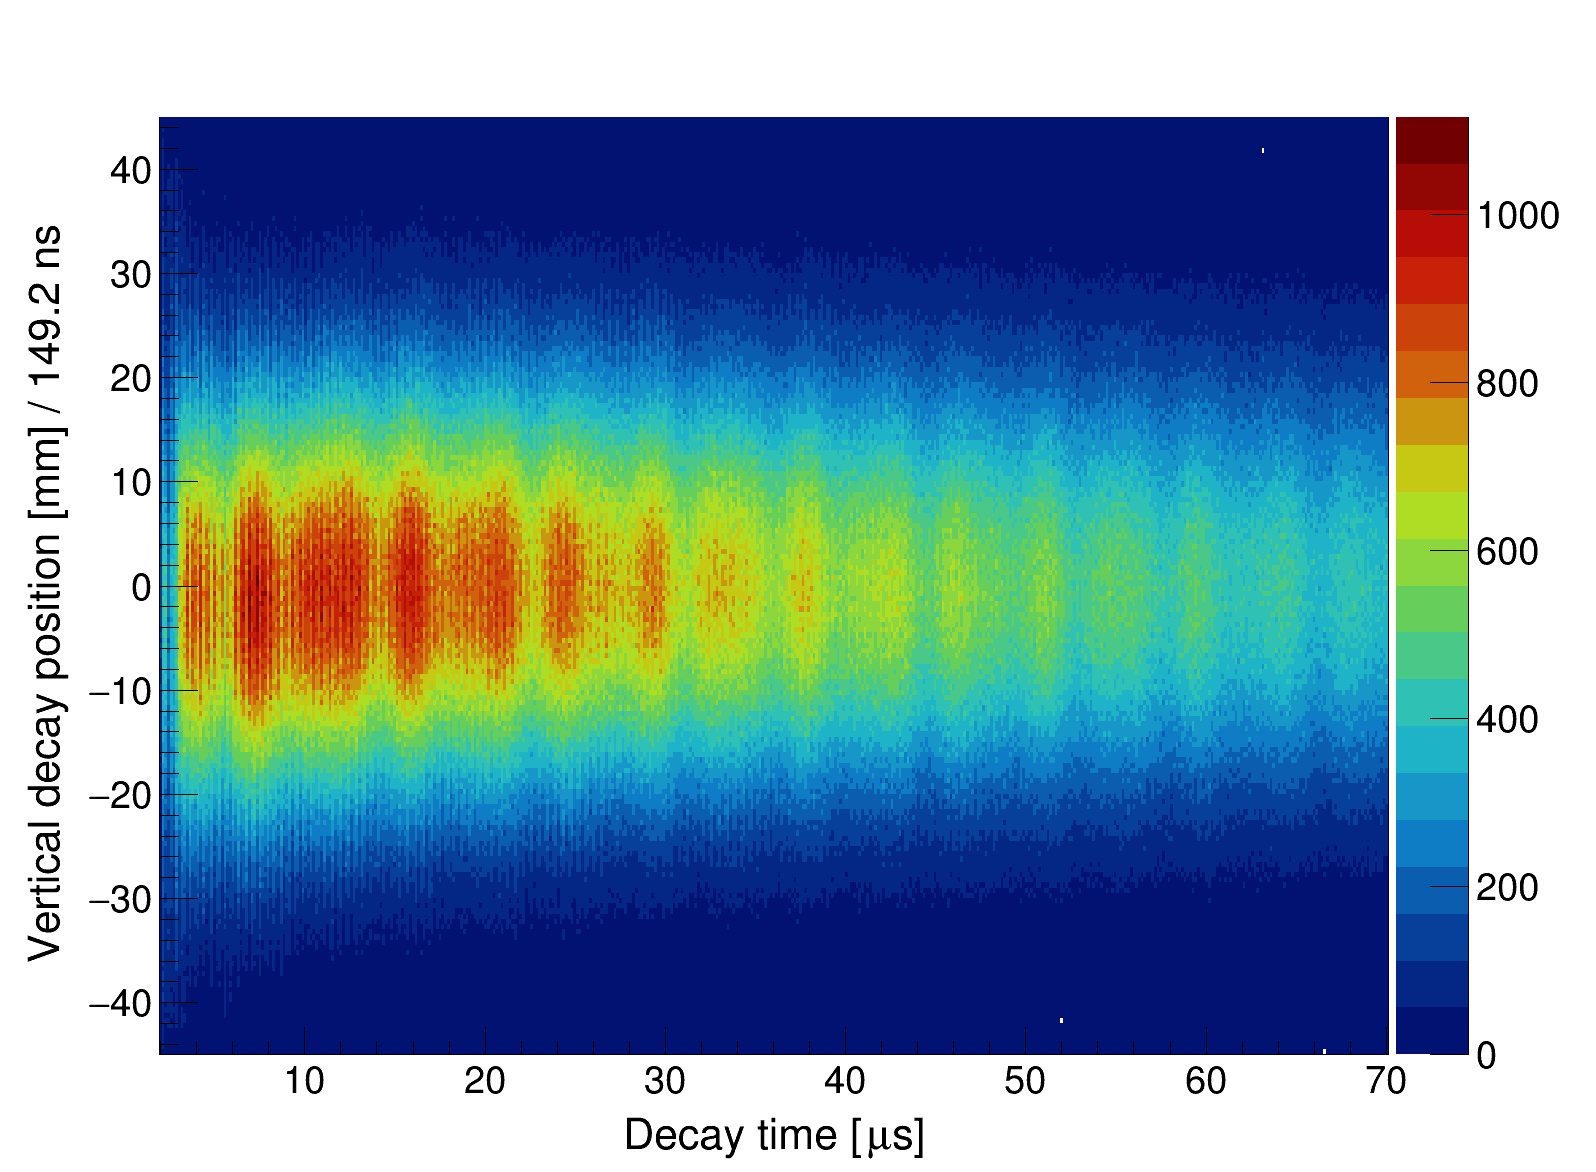
\includegraphics[trim={0 0 0 0},clip,width=.49\textwidth]{Images/Chapter3/Y_vs_t.png}}
\caption{Coherent betatron oscillations as measured by the straw trackers described in Section \ref{subsec:Trackers}. The vertical oscillation has an observed frequency which is much higher than its radial counterpart, and so is more difficult to see.}
\label{fig:CBO}
\end{figure} 
\begin{figure}[t!]
\centering{}
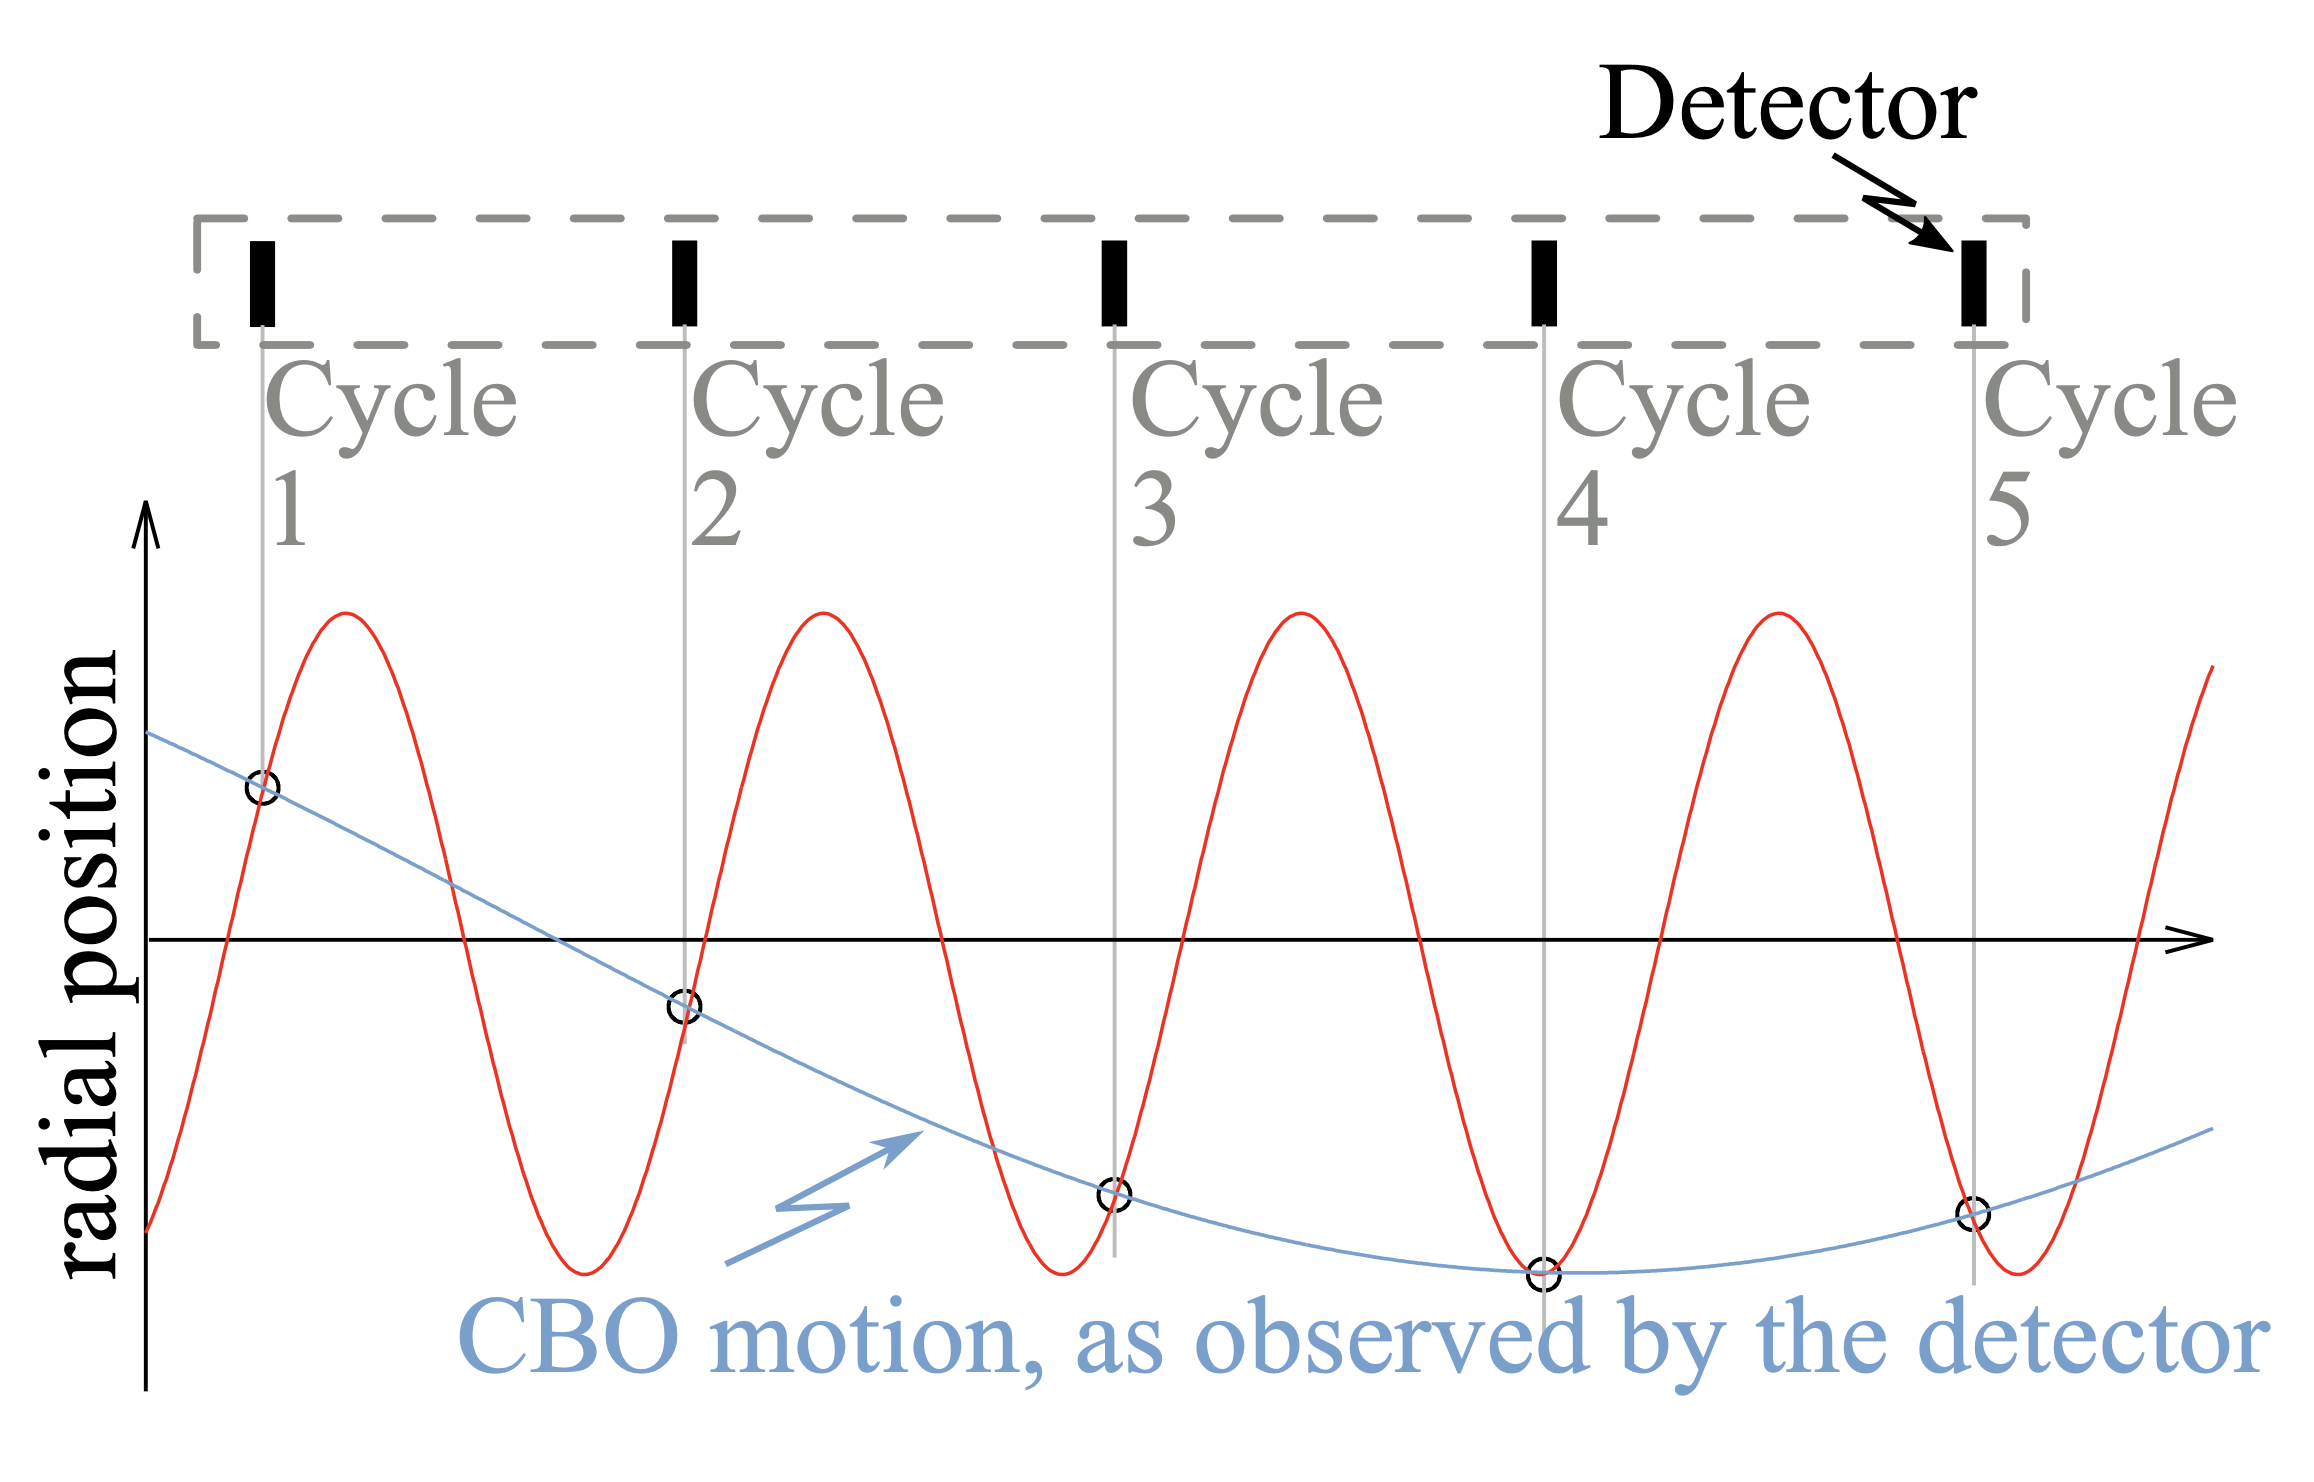
\includegraphics[trim={0 0 0 0},clip,width=.59\textwidth]{Images/Chapter3/CBO_diagram.png}
\caption{The aliasing of the observed frequency of an oscillation. Image reproduced from \cite{KimCBO}.}
\label{fig:Aliasing}
\end{figure} 

For an oscillation with a frequency $f$, where $f$ is greater than $f_{c}/2$ (the Nyquist frequency \cite{Nyquist}), the observed frequency of that oscillation will be aliased to the beat frequency $f_{c} - f$, as explained by Figure \ref{fig:Aliasing}. This is the case with the radial betatron frequency, $f_{x}$, which has an observed CBO motion which is much slower than the underlying betatron oscillation, at a frequency 
%
\begin{equation}
  f_{\text{CBO}_{x}} = f_{c}-f_{x}.
  \label{eqn:CBOx}
\end{equation}
%
One further important oscillation in the average width of the beam, with a frequency of $2\cdot f_{y}$, is called the `vertical waist' (VW). The frequency the VW is aliased to 
%
\begin{equation}
  f_{\text{VW}} = f_{c}-2\cdot f_{y}.
  \label{eqn:VQ}
\end{equation}

The EDM search described in this thesis relies on measuring an oscillation in the vertical decay angle modulated at the anomalous precession period, which has a frequency $f_{a}$. Both the CBO and VW oscillations occur at higher frequencies than $f_{a}$, so must be considered in the analysis. Important beam oscillations at E989 are summarised in Table \ref{tbl:Frequencies}. Further information on the CBO and VW can be found in \cite{BeamDynamics} and \cite{KimCBO}.

\begin{table}[t!]
\centering
\begin{tabular}{l|ccc}
\hline
\hline
Quantity & Expression & Frequency [MHz] & Time period [\SI{}{\micro\second}] \\
\hline
Anomalous precession & $f_{a}$ & 0.229 & 4.365 \\
Cyclotron & $f_{c}$ & 6.71 & 0.1492 \\
Horizontal betatron & $f_{x}=f_{c}\cdot\sqrt{1-n}$ & 6.34 & 0.158 \\
Vertical betatron & $f_{y}=f_{c}\cdot\sqrt{n}$ & 2.21 & 0.452 \\
Coherent betatron oscillation & $f_{\text{CBO}_{x}} = f_{c}-f_{x}$ & 0.37 & 2.703 \\ 
Vertical waist & $f_{\text{VW}} = f_{c}-2\cdot f_{y}$ & 2.31 & 0.433 \\
\hline
\hline
\end{tabular}
\caption{A summary of muon beam oscillation frequencies in the E989 experiment \cite{TDR}. The values presented here correspond to an $n$ value of 0.108, or a voltage of \SI{18.3}{\kilo\volt}, which was used in two of four Run-1 datasets (Run-1a and Run-1d), as detailed in Section \ref{sec:MeasPeriods}.} 
\label{tbl:Frequencies}
\end{table}%18.3 kV for all datasets except Run-1b and Run-1c, where it is 20.4 kV

\subsection{The fast rotation}\label{subsec:FR}

The rotation frequency of a stored muon is approximately inversely proportional to its equilibrium radius, $x_{e}$, which is relative to $R_{0}$. This means that, following injection as a bunch, muons at smaller radii will begin to overtake those at greater radii: causing de-bunching as the beam revolves around the storage ring. This result is a rapid modulation of the cyclotron frequency early in the fill, which largely dies away after \SI{30}{\micro\second} once the muons are uniformly distributed around the ring. This `fast rotation' (FR) effect, showing in Figure \ref{fig:FR}, necessitates a correction to $\omega_{a}$ \cite{OmegaARun1}, but in the context of the EDM search the fast rotation effect is removed by a combining data in intervals equal to the cyclotron period, $T_{c}$, and then applying uniform randomisation of decay times at $\pm T_{c}/2$ (discussed further Chapter \ref{chap:6} Section \ref{subsec:BeamDynamicsCorr}). Further information on the FR can be found in \cite[and references therein]{BeamDynamics}.

\begin{figure}[t!]
\centering{}
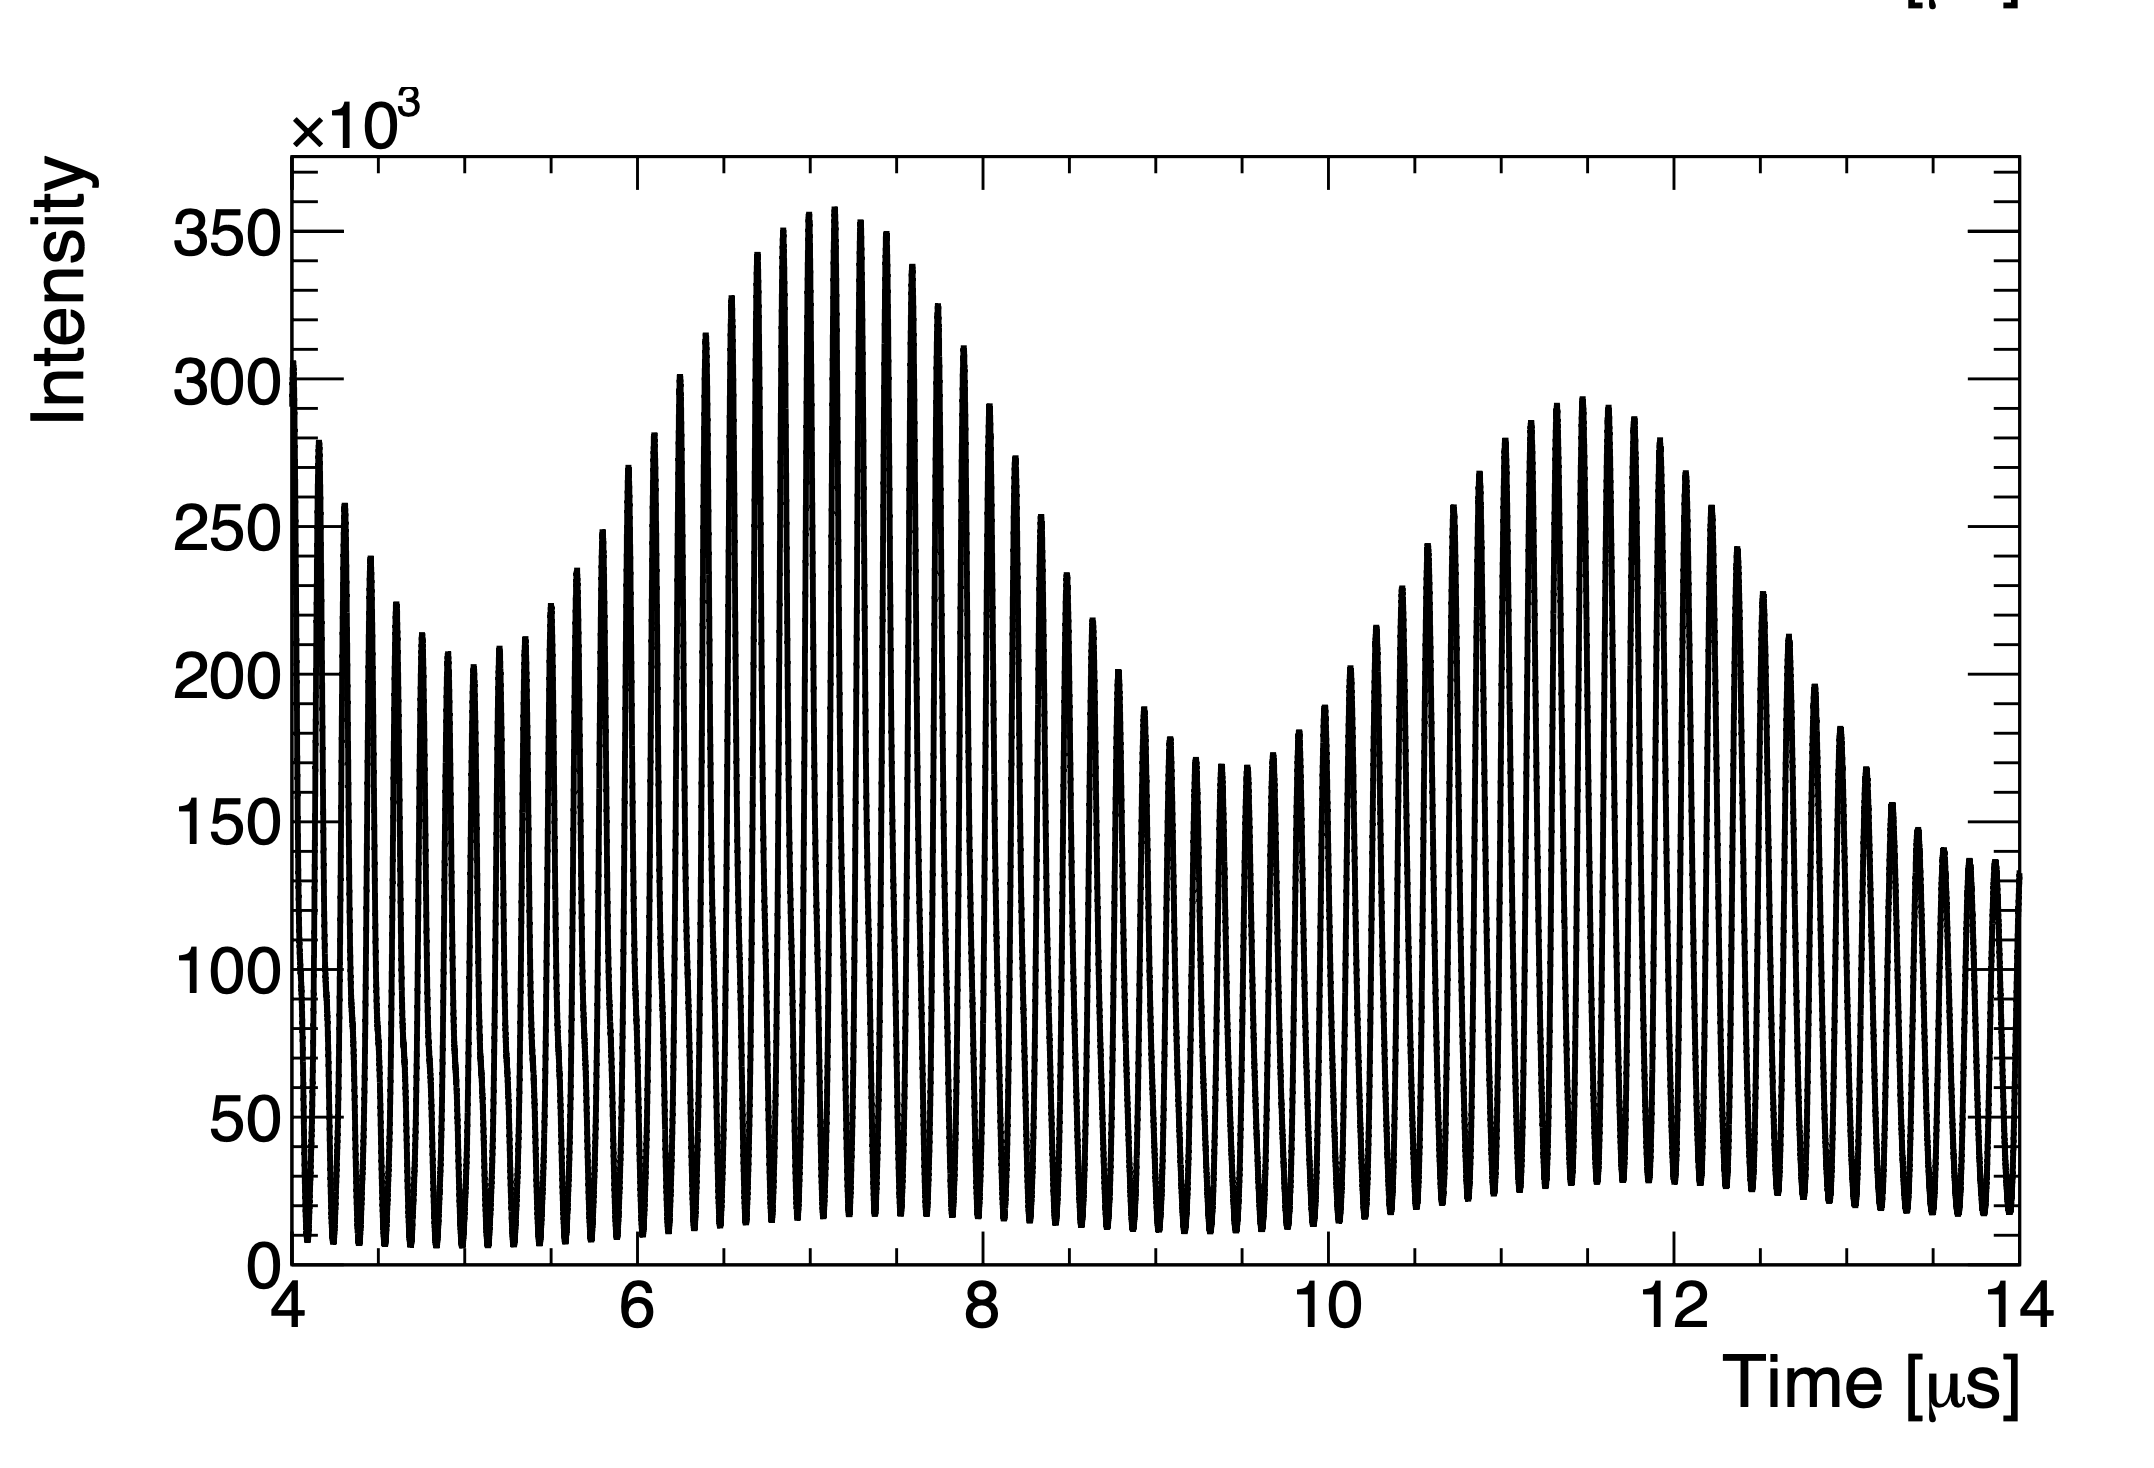
\includegraphics[trim={0 0 0 0},clip,width=.69\textwidth]{Images/Chapter3/FR.png}
\caption{The positron number oscillation early in the fill, counted in intervals of 1 ns, showing the rapid oscillation caused by the fast rotation effect. The modulation of the amplitude is caused by $\omega_{a}$. Image reproduced from \cite{BeamDynamics}.}
\label{fig:FR}
\end{figure} 

\begin{figure}[t!]
\centering{}
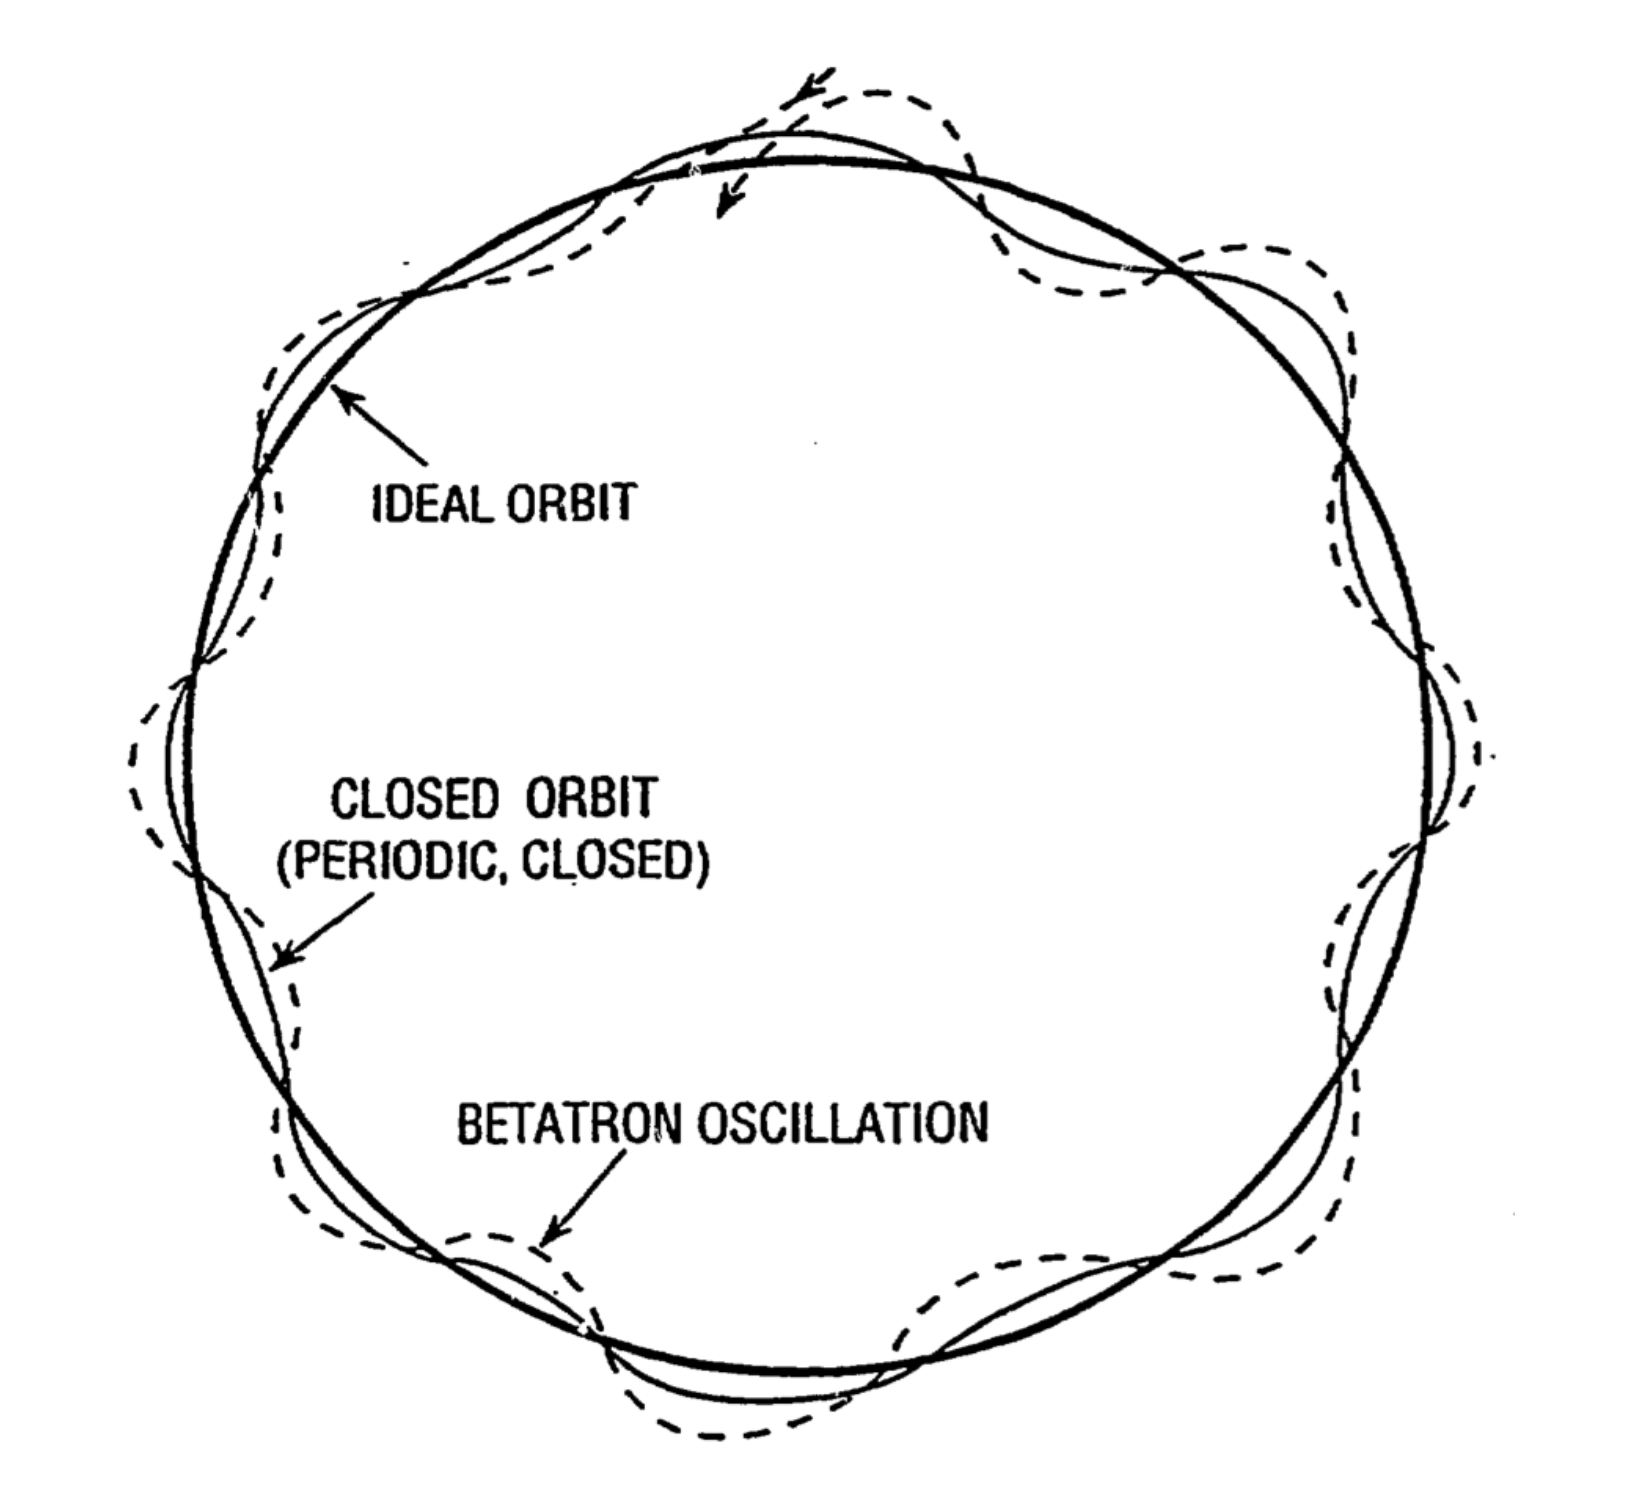
\includegraphics[trim={0 0 0 0},clip,width=.59\textwidth]{Images/Chapter3/COD_cartoon.png}
\caption{An illustration of the radial closed orbit, where the beam equilibrium radius is periodically displaced from the ideal orbit. The horizontal betatron oscillation is also indicated by a dashed line. Imaged reproduced from \cite{COD_note}.}
\label{fig:COD}
\end{figure} 

\subsection{The distortion of the closed orbit}\label{subsec:COD}

Local inhomogeneities in the storage ring magnetic field cause the equilibrium radius of the beam to vary as function of ring azimuthal angle, culminating in an effect termed the `closed orbit distortion' (COD). An illustration of the radial closed orbit is shown in Figure \ref{fig:COD} \cite{COD_note}.

Variations in the vertical electric field, and radial magnetic field, also result in a vertical COD. This effect is highly relevant to the radial magnetic field measurements presented in Chapter \ref{chap:4}, and is discussed in detail in Section \ref{sec:VCOD} of that chapter.

\section{The magnetic field}\label{sec:Field}

The E989 magnetic field system consists of the superconducting magnetic storage ring (referred to here as the `main magnet'), a suite of NMR probes used to map the magnetic field, and an array of passive and active of shims used to reduce inhomogeneities in the field. The system is designed to produce a vertical magnetic field of 1.45 T, with uniformity of 1 part-per-million (ppm) around the full azimuth of the muon storage region.

The main magnet, originally designed and built for the E821 $g-2$ experiment at BNL, is a continuous ring of low-carbon steel which is excited by superconducting coils to generate a magnetic field. Twelve flux return yokes, each covering a 30{\degree} azimuthal section, are fixed together to form a ring approximately 15 m in diameter and 3 m high, with a mass of 680 metric tons. Each yoke has a `C-shaped' cross-section, illustrated by Figure \ref{fig:Magnet}, which partially encloses the muon storage region, and allows decay positrons to exit the field in the direction of the ring interior. 

Magnetic flux is induced in the yokes by three superconducting niobium-titanium (NbTi) coils connected in series, which carry a $\sim$5170 A current from a 5 V power supply. There is one outer coil and two inner coils, positioned on either side of the equilibrium radius of the storage region, $R_{0}=7112$ mm, at radii of 6677 mm and 7512 mm respectively. The outer coil, consisting of 48 turns with a gap at the mid-plane to allow space for the inflector, drives the field across the storage region; the two inner coils, consisting of 24 turns each, are supplied with a current in the opposing direction to the outer coil, cancelling the flux in the ring centre and improving the quality of the field in the storage region. The coils are typically operated at temperature of \SI{5}{\kelvin}, which is maintained by a supply of cryogenic helium.
%
\begin{figure}[t!]
\centering{}
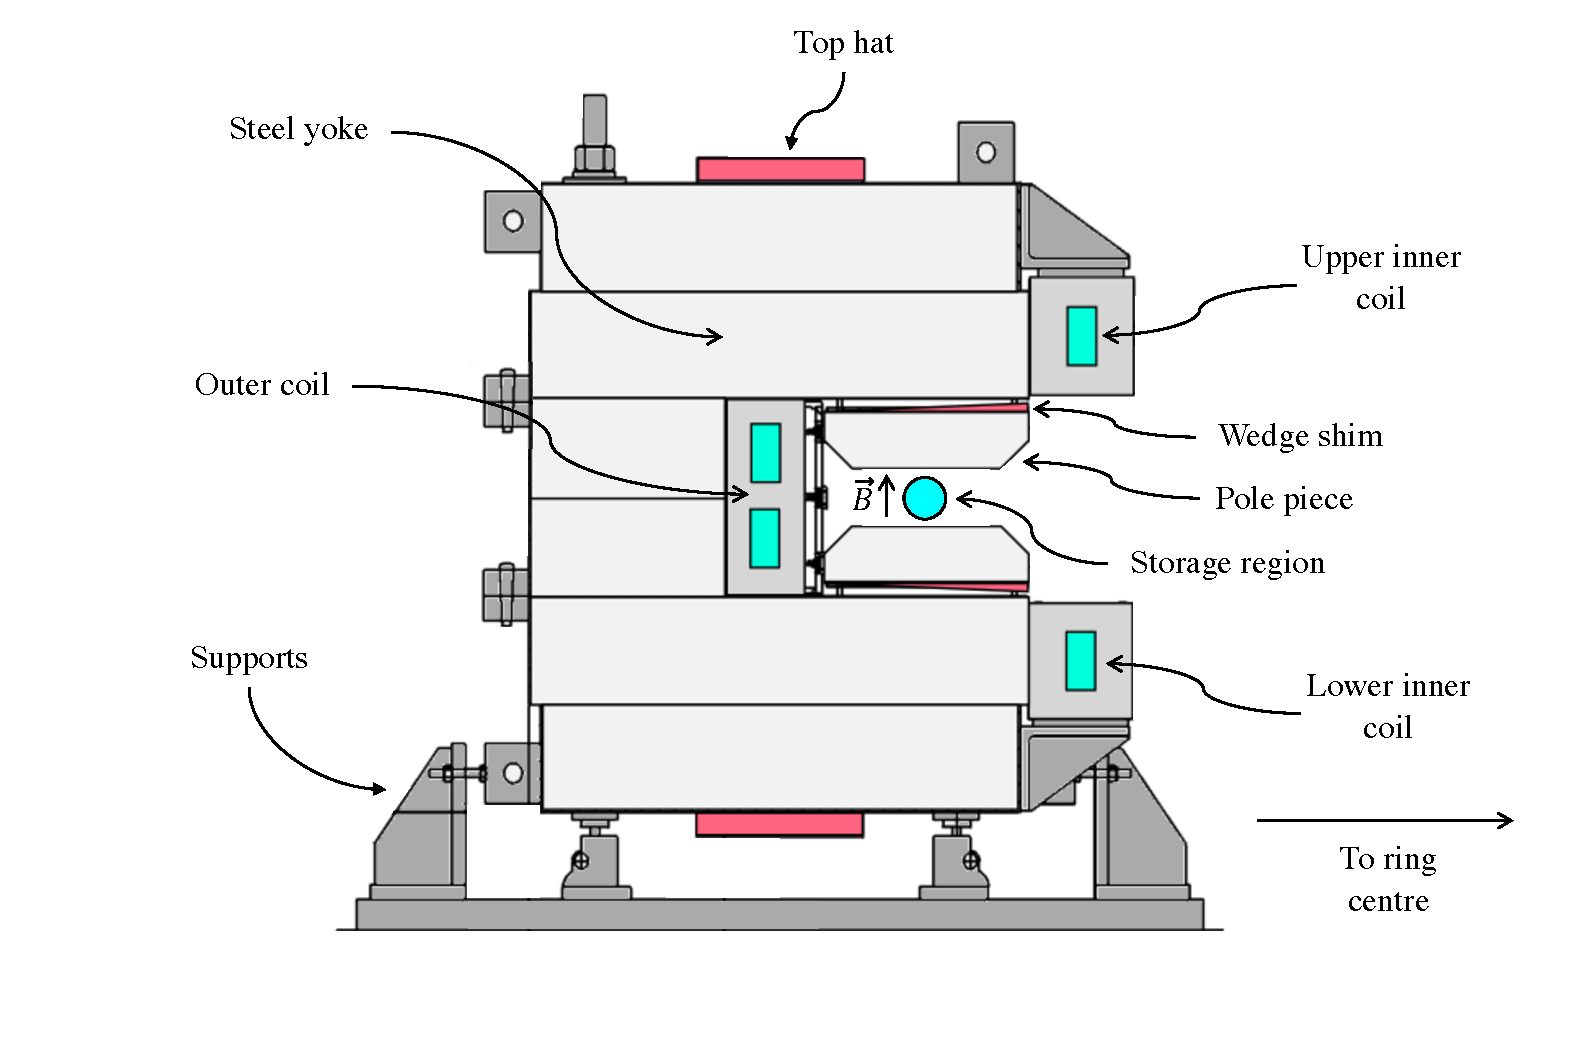
\includegraphics[trim={0 0 0 0},clip,width=\textwidth]{Images/Chapter3/BNLMagnetCrossSection4.pdf}
\caption{A cross-section of the E989 main magnet, showing: the `C-shaped' yoke, superconducting coils (green), pole pieces, shims (red), and muon storage region (blue). The orientation of the magnetic field in the storage region is indicated by an arrow. Not shown are the additional passive shims, and the surface correction coils (active shims), fixed to the inner surfaces of the pole pieces. Image adapted from Figure 2 of \cite{BNLMagnet}, and inspired by Figure 2.4 of \cite{Sweigart}.}
\label{fig:Magnet}
\end{figure} 

The dipole field across the storage region is shaped by sections of higher quality steel called `pole pieces'. The pole pieces are isolated from the magnet bulk an air gap of \SI{1.5}{\centi\metre}, decoupling the field across the storage region from aberrations in the yoke and producing a highly uniform field. The air gap also allows space for steel wedges to be inserted, which, along with larger sections of steels fixed to the top and bottom of the yoke called `top hats', improve uniformity of the field by passive shimming. Additional `edge shims' on the inner surfaces of pole pieces, as well as iron foil laminations, fine-tune the field uniformity even further. The process of mechanically shimming the magnetic field was carried out during the E989 commissioning period in 2015-2016, reducing variations in the field to within $\sim$100 ppm, as shown in Figure \ref{fig:ShimmingResults}. Detailed discussion of the shimming campaign can be found in \cite{Smith}.

The azimuthally averaged variations in the field are finally brought to within $\sim$1 ppm by the active shimming provided by sets of 100 concentric current-carrying coils, which are printed on circuit boards and fixed to the inner surface of the each pole piece. The currents carried by these `surface correction coils' (SCCs), may be adjusted during operation by input in the stand-alone magnetic field DAQ system. This utility of this subsystem, beyond shimming the magnetic field, will be demonstrated in Chapter \ref{chap:4}.

Finally, the muon storage region is enclosed in an aluminium vacuum chamber, in order to both prevent the beam from scattering off air molecules and to minimise the likelihood of discharge from any of the various high voltage systems inside the ring. Detailed discussion on the main magnet can be found in \cite{TDR} and \cite{BNLMagnet}.
%
\begin{figure}[t!]
\centering{}
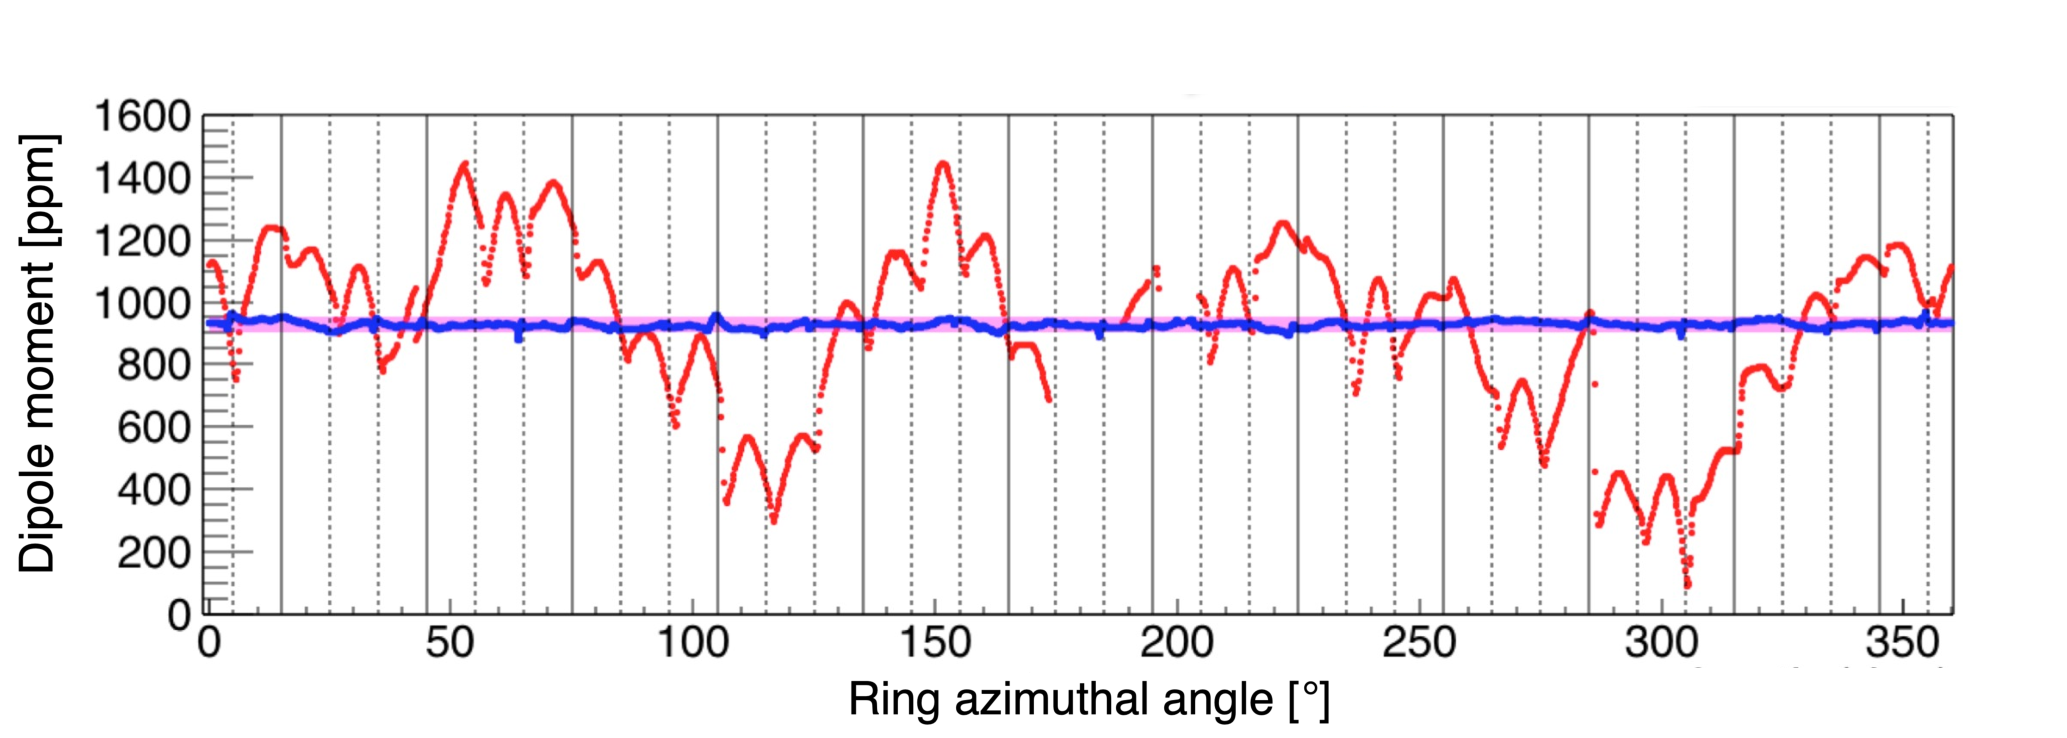
\includegraphics[trim={0 0 0 0},clip,width=.89\textwidth]{Images/Chapter3/ShimmingPlot.pdf}
\caption{The dipole magnetic field measured around the ring before the shimming campaign in 2015-2016 (red) and after (blue), where variations in the field were reduced to $\sim$100 ppm. Image adapted from \cite{ShimmingTalk}.}
\label{fig:ShimmingResults}
\end{figure}

\begin{figure}[t!]
\centering{}
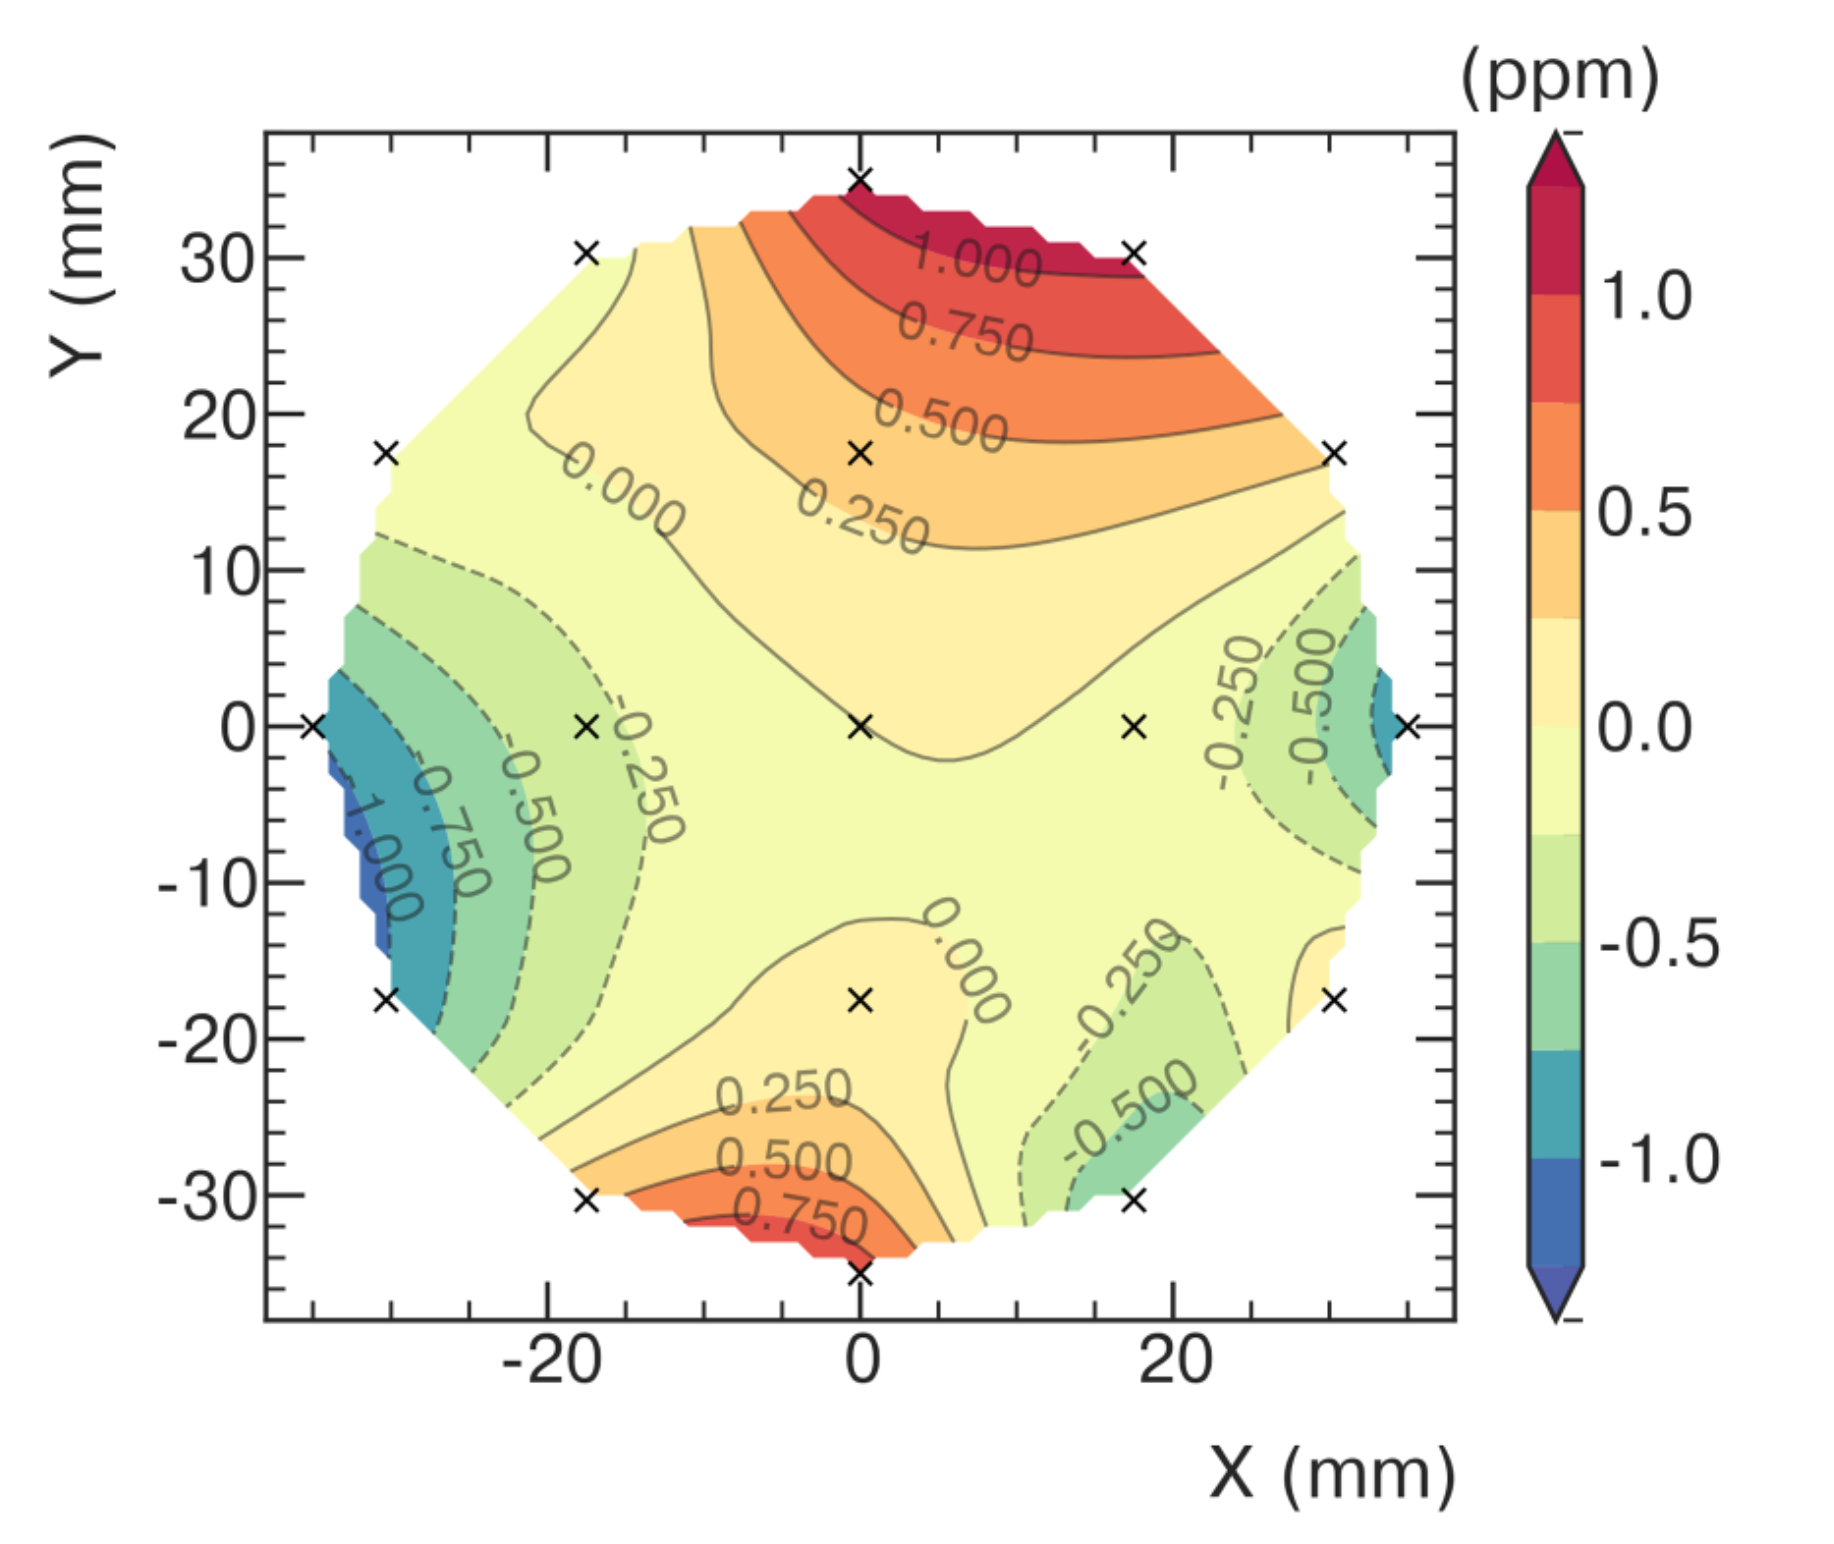
\includegraphics[trim={0 0 0 0},clip,width=.69\textwidth]{Images/Chapter3/TrolleyMap.png}
\caption{An azimuthally averaged field map of the storage region, constructed from data taken from a single trolley NMR probe. Variations in the magnetic field are within the target $\sim$1 ppm. Image reproduced from \cite{Field}.}
\label{fig:Trolley}
\end{figure}

The magnetic field is measured by 378 fixed NMR probes attached to the top and bottom of the vacuum chamber, called `fixed probes', and a mobile array of 17 NMR probes which periodically transits the full circumference of vacuum chamber in a device called the `trolley'. Each probe contains a sample of a proton rich organic substance (petroleum jelly), where the Larmor precession frequency of the protons in the substance is proportional to the strength of the field. The probes are calibrated by comparison with measurements taken with a device termed the `plunging probe', which contains a sample of well-characterised high purity water. The fixed probes provide a means of measuring the field drift while the experiment is receiving beam, while the trolley is used to build precision maps the field from several thousand points around the ring during dedicated beam-off periods called `trolley runs', which take place every three days. An example of an azimuthally averaged field map produced by a single trolley probe is shown in Figure \ref{fig:Trolley}. The field maps from the trolley are weighted with maps of the spatial beam distribution measured by the straw tracking detectors, discussed in Section \ref{subsec:Trackers}, in order to measure the average magnetic field experienced by the muons at the time of decay.
%
\section{Detectors}\label{sec:Detectors}

\subsection{Auxiliary detectors}\label{subsec:Aux}

The auxiliary detectors are distinct from the calorimeters and straw tracking detectors, which are discussed in the following sections, in that their function relates to making direct measurements of the muon beam in order to monitor injection and study beam dynamics, rather than detecting decay positrons. 

\begin{figure}[t!]
\centering{}
\subfloat[T0]{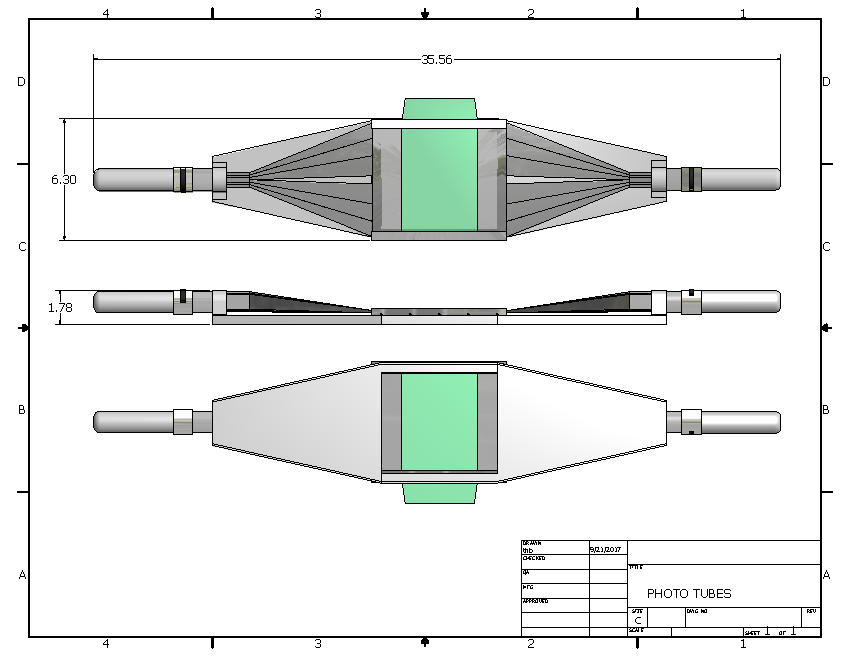
\includegraphics[trim={0 0 0 0},clip,width=.33\textwidth]{Images/Chapter3/T0.pdf}}\hfill
\subfloat[IBMS]{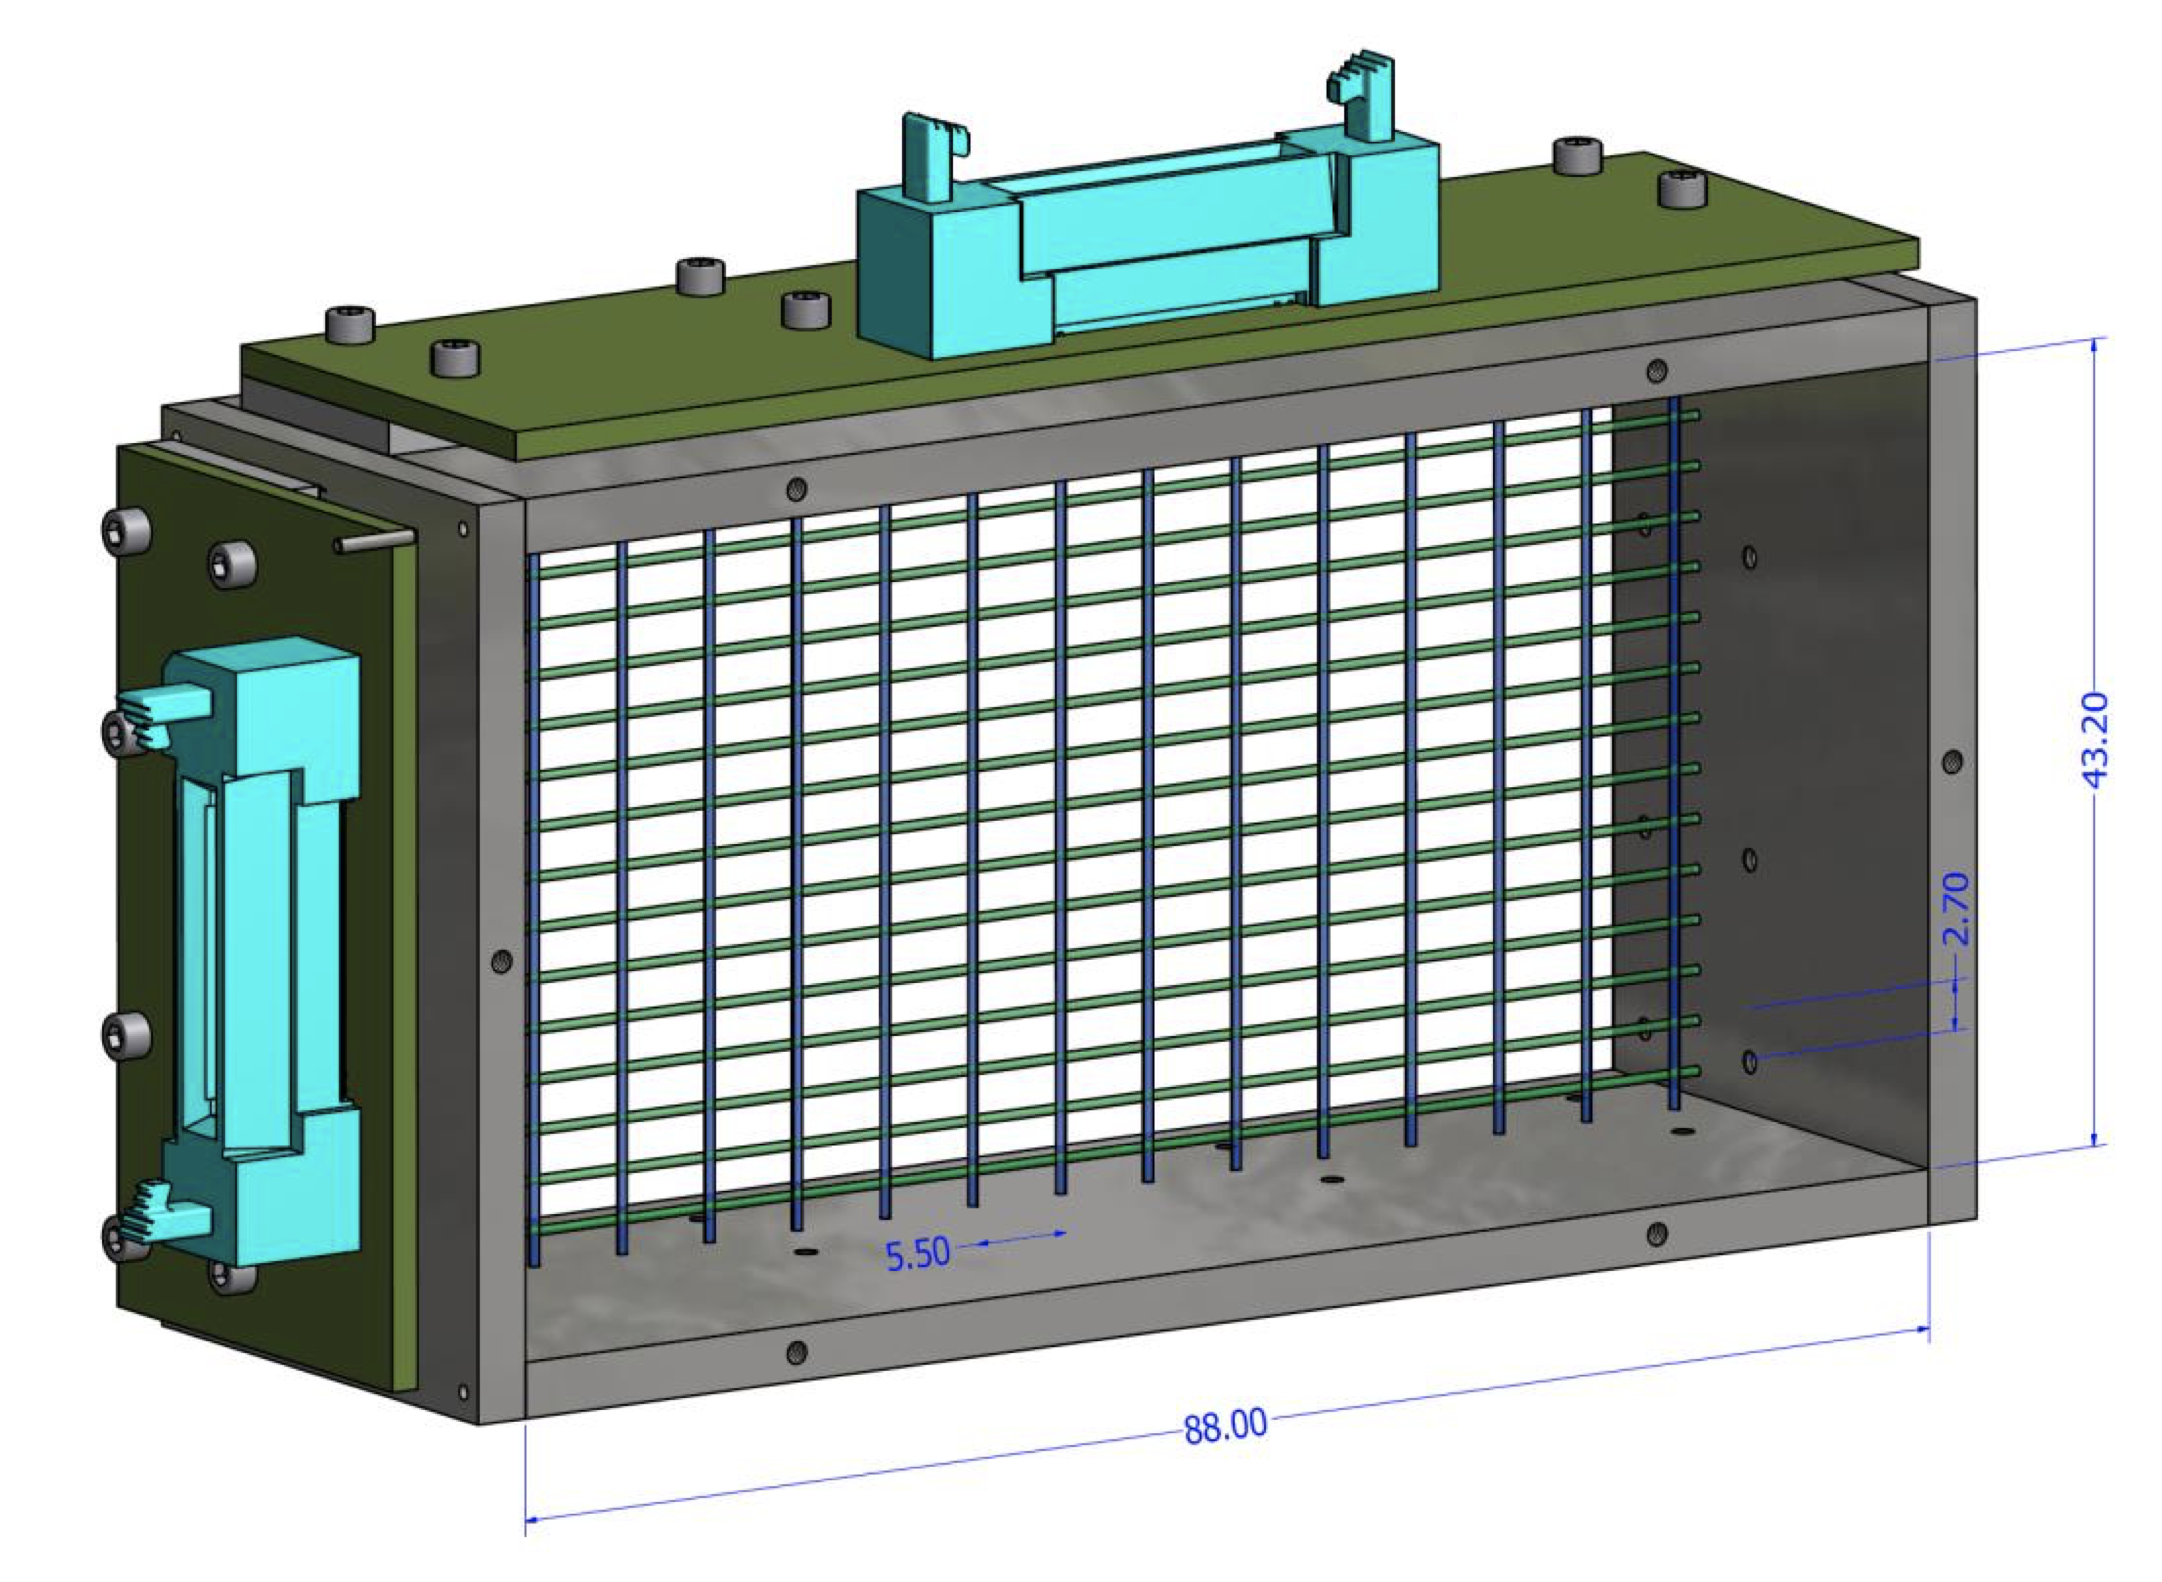
\includegraphics[trim={0 0 0 0},clip,width=.33\textwidth]{Images/Chapter3/IBMS1.png}}\hfill
\subfloat[Fibre harp]{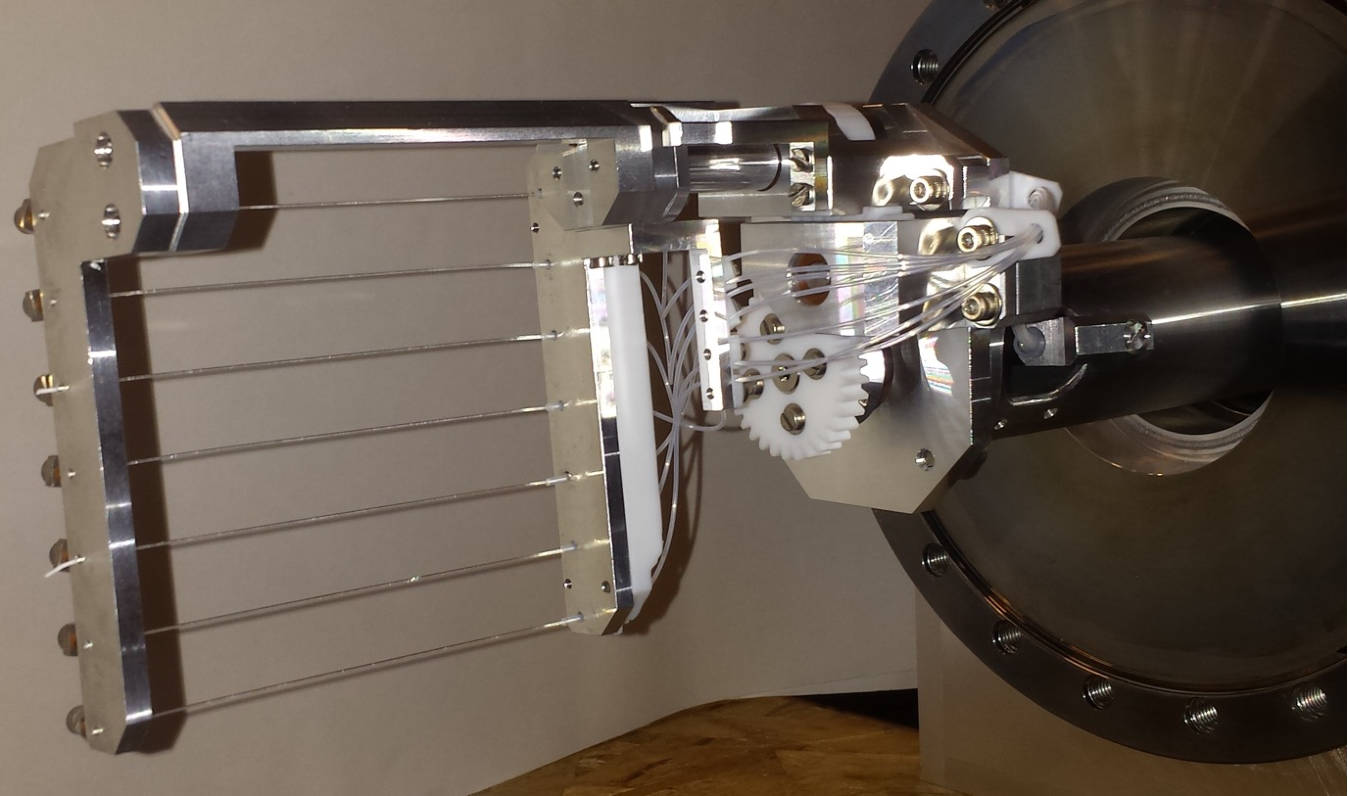
\includegraphics[trim={0 0 0 0},clip,width=.33\textwidth]{Images/Chapter3/FiberHarp.pdf}}
\caption{Representations of the E989 auxiliary detector systems, showing: (a) a schematic of the T0 counter, showing the scintillator (green) attached to PMTs on the left and right; (b) a computer model of one the IBMS detectors (IBMS1), showing the grid of scintillating fibres connected to SiPMs; (c) a photograph of one of the four fibre harps, showing the scintillating fibres (horizontally aligned in this case) mounted on a retractable arm. Images reproduced from \cite{T0}, \cite{IBMS}, and \cite{FibreHarpPoster}.}
\label{fig:AuxDetectors}
\end{figure} 

Three systems fall into this category, the first being the `T0' counter: a scintillating paddle connected to two photomultiplier tubes (PMTs), positioned outside the ring and upstream of the inflector. The primary function of the T0 is to define the initial time of the fill, $t=0$, which is essential for the synchronisation the various systems in the ring \cite{T0}. The second auxiliary detector is the `inflector beam monitoring system' (IBMS): grids of scintillating fibres connected to silicon photomultipliers (SiPMs), positioned at two locations upstream of the inflector. The IMBS measures the spatial distribution of the muons before injection, providing the valuable diagnostic information required for optimally directing the beam through the narrow inflector aperture. An additional IBMS detector with horizontal fibres only may be inserted downstream of the inflector to make a destructive measurement of the vertical beam profile \cite{IBMS}. The third of these systems are the `fibre harps', which were recovered from the E821 $g-2$ experiment and refurbished for use in E989. These are retractable `harps' of scintillating fibres, which can be inserted inside the vacuum chamber at approximate ring azimuthal angles of 180$\degree$ and 270$\degree$. Two detectors are positioned at each location, one with horizontally aligned fibres and another with vertically aligned fibres. While inserted, the fibre harps are used to make a destructive measurement of the spatial distribution of the beam, serving as a means of directly measuring effects such as the horizontal and vertical CBO during dedicated systematic runs. More information on the fibre harps may be found in \cite{TDR}. 

\subsection{Calorimeters}\label{subsec:Calos}

The primary means of positron detection at E989 are the twenty-four electromagnetic calorimeters which instrument the interior the ring, indicated by numbers 1 through 24 in Figure \ref{fig:RingSchematic}. The purpose of the calorimeters is to measure the energy, arrival time, and (to a lesser extent) the hit position of decay positrons.

\begin{figure}[t!]
\centering{}
\subfloat[]{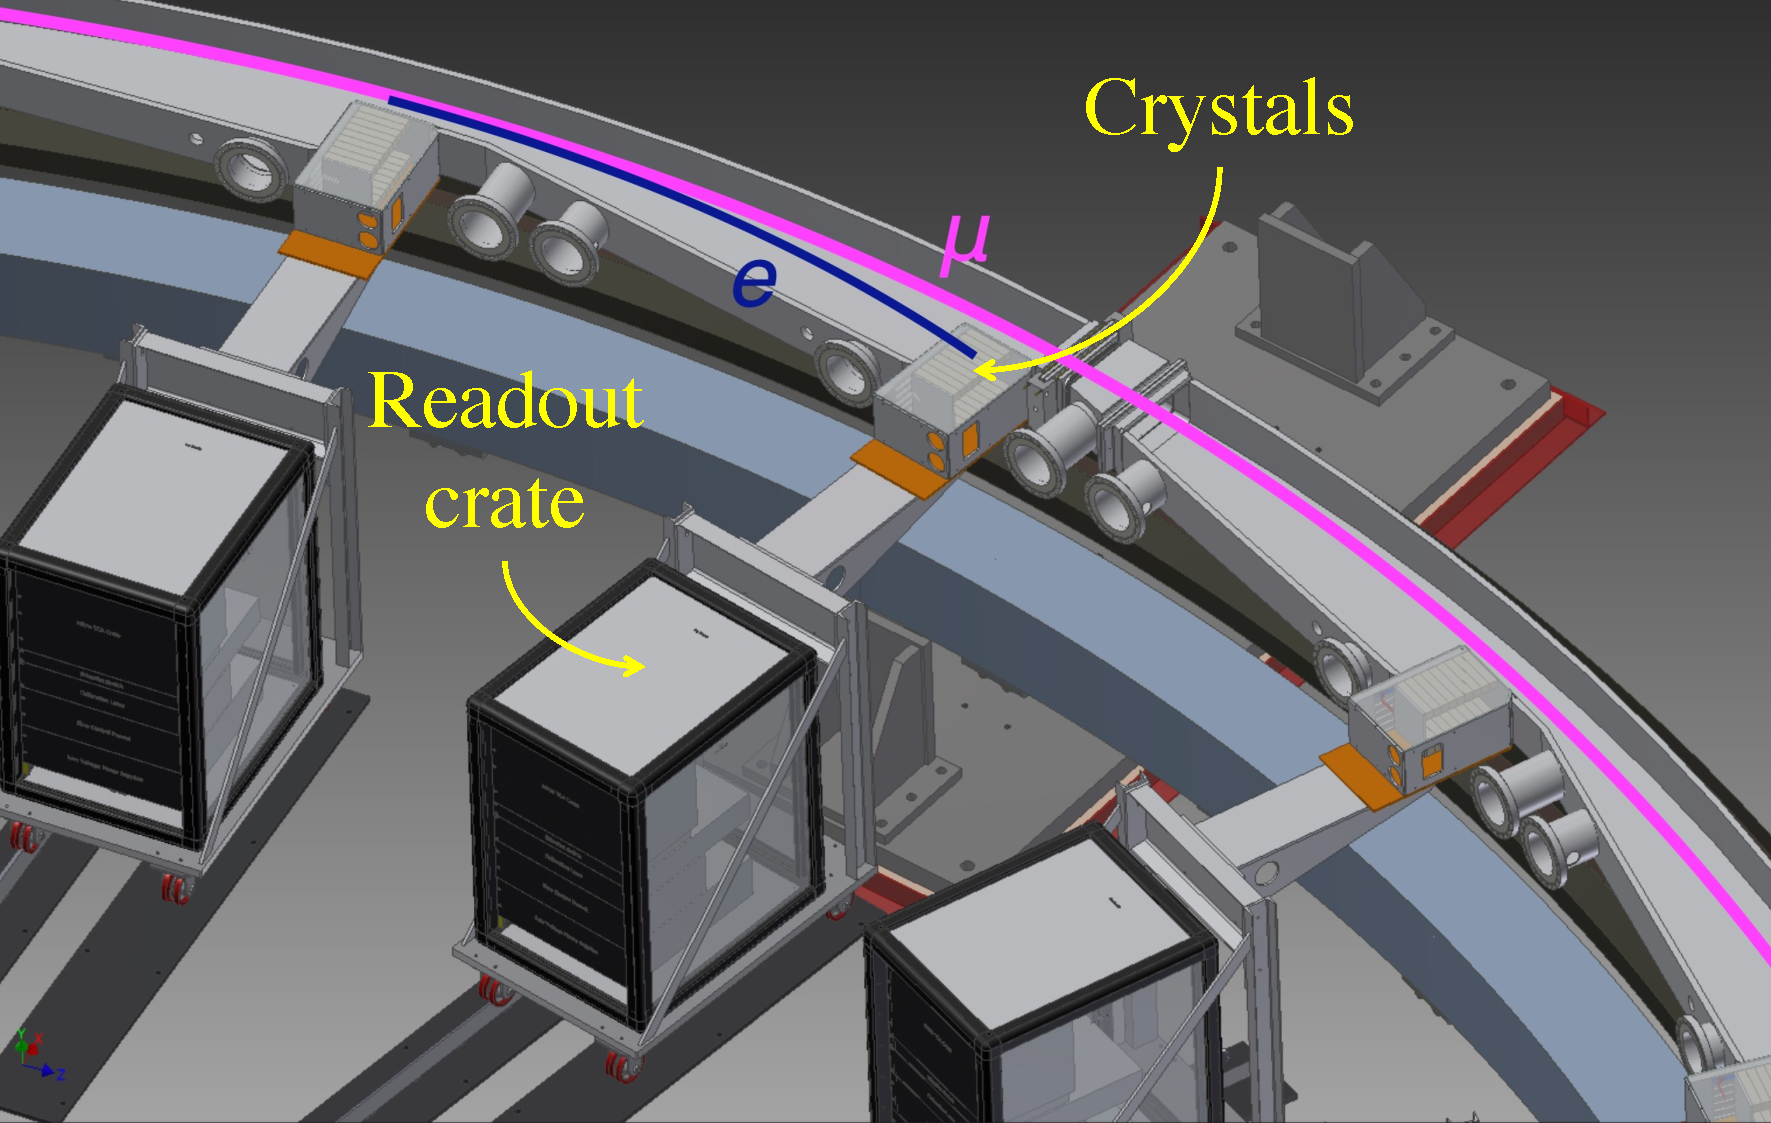
\includegraphics[trim={0 0 0 0},clip,width=.69\textwidth]{Images/Chapter3/CaloIllustration.pdf}\label{subfig:CaloModel}}
\hfill
\subfloat[]{\includegraphics[trim={0 1.2cm 0 0},clip,width=.69\textwidth]{Images/Chapter3/CaloCrystals.png}\label{subfig:CaloCrystals}}
\caption{The E989 calorimeters, showing: (a) a model of three calorimeters in position during operation, with an incident decay positron indicated by a blue line; (b) a photograph of the $\text{PbFl}_{2}$ crystals and SiPMs during assembly. Images reproduced from \cite{CaloCommissioning}.}
\label{fig:Calos}
\end{figure} 

Unlike the E821 calorimeters, which had a monolithic construction, the E989 calorimeters are composed of a segmented $9\text{-wide}\times6\text{-high}$ array of lead-fluoride ($\text{PbFl}_{2}$) crystals, a each with a volume of $25\times25\times140$ $\text{mm}^3$. Behind every crystal is a silicon photomultiplier (SiPM), which senses the Cherenkov light produced by relativistic charged particles passing through the crystal medium. The intensity of the light falling onto the SiPMs is proportional to the incident positron energy. Each crystal is isolated from its neighbours by a thin opaque and non-reflective wrapping, black Tedlar foil, which greatly limits the level of light transmitted between crystals: improving the spatial resolution of detected hits. The calorimeters are spaced evenly around the ring, each positioned immediately downstream of an extruded section of the vacuum chamber -- allowing decay positrons to travel with minimal energy loss before exiting the vacuum and being intercepted. Frontend electronics for each calorimeter are housed in a crate positioned away from the magnetic field region. A illustration of the calorimeters in position relative to the vacuum chamber is shown in Figure \ref{subfig:CaloModel}, and a photograph of the $\text{PbFl}_{2}$ crystals is shown in Figure \ref{subfig:CaloCrystals}. 

The calorimeter temporal resolution exceeds \SI{100}{\pico\second} for positrons with a kinetic energy greater than 100 MeV, as specified by the design requirements \cite{TDR}, aided by the short and fast signal produced by Cherenkov radiation. This requirement is motivated by the need to resolve pileup events, where two or more hits close in time and space are erroneously reconstructed as a single hit. Pileup, if unresolved, changes the number of positrons detected `above threshold' in the $\omega_{a}$ number oscillation. Pileup is more prominent early in the fill, causing an apparent time dependence in the phase of $\omega_{a}$. The requirements of the energy resolution of the calorimeters are less stringent, at better than 5\% at 2 GeV, since the $\omega_{a}$ measurement only uses the hit cluster energy as means of event selection rather than as a direct observable. 

An additional requirement on the calorimeters is that variations in the energy response, or gain, must fall within 0.1\% per \SI{200}{\micro\second}. Much like pileup, changes in gain can bias $\omega_{a}$ between early and late times in the fill. To monitor this, a system of lasers periodically fire pulses of light into the crystals, allowing for `in-fill' gain variations to be corrected by directly comparing the detected energy to the energy deposited by the laser. The laser monitoring system may also be used to detect gain variations fill-by-fill, as well as to measure the SiPM time resolution by firing two pulses in quick succession. Detailed discussion on the calorimeters may be found in \cite{TDR} and \cite{Hempstead}.

\subsection{The straw trackers}\label{subsec:Trackers}

The straw trackers, or trackers, are a secondary system of positron detectors which are designed to make a non-destructive measurement of muon beam profile, reconstructing both the decay position and momentum of particles exiting the storage region as a function of time.

The information provided by the trackers is extremely valuable for a numbers of reasons. Firstly, it enables the precise characterisation of beam dynamics effects such a betatron motion, described in Section \ref{sec:BeamDynamics}, minimising the associated systematic uncertainty on $\omega_{a}$. Secondly, and as discussed in Section \ref{sec:Field}, tracker measurements of the spatial beam distribution are used to weight the field maps measured by the trolley NMR probes, which is essential for the final determination of the magnetic field. Thirdly, positron trajectories may be extrapolated both backwards to the point of decay, or forwards to the downstream calorimeter: enabling direct comparison between tracker hits, hereafter referred to as `tracks', and calorimeter clusters. This `tracker-calorimeter matching' is extremely useful for cross-checks of pileup and gain variations\footnote{A study utilising tracker-calorimeter matching (conducted by the author), where the ratio of cluster energy to track momentum was used to verify gain measurements made by the laser monitoring system, can be found in \cite{EpNote}.}. Finally, the trackers' ability to measure the time evolution of the average positron vertical decay angle is central to the muon EDM search described in this thesis.

\begin{figure}[t!]
\centering{}
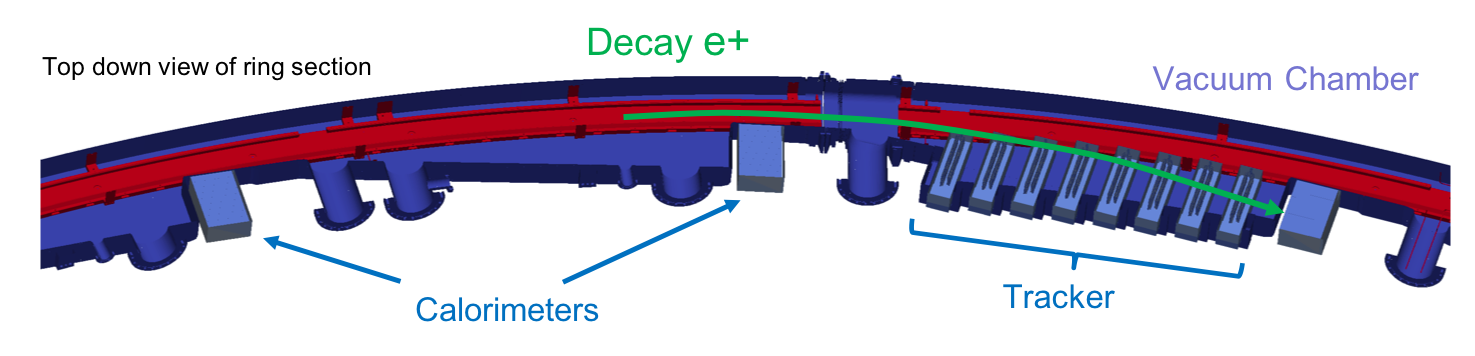
\includegraphics[trim={0 0 0 0},clip,width=\textwidth]{Images/Chapter3/TrackerVacChamber.png}
% \subfloat[]{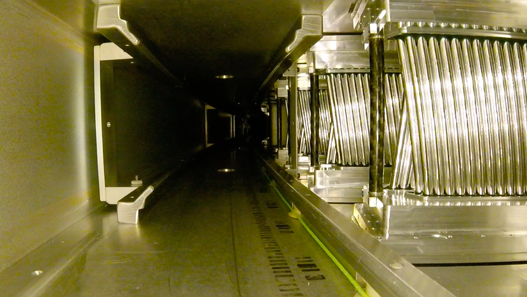
\includegraphics[trim={0 0 0 0},clip,width=.49\textwidth]{Images/Chapter3/Tracker-InVac.png}}
\caption{A rendering of the tracker modules in position inside the vacuum chamber, shown with respect to nearby calorimeters. The trajectory of a decay positron is shown in green, illustrating the case where a track may be matched with a calorimeter cluster. Image courtesy of the E989 collaboration.}
\label{fig:TrackerSchematic}
\end{figure} 

\begin{figure}[t!]
\centering{}
\subfloat[]{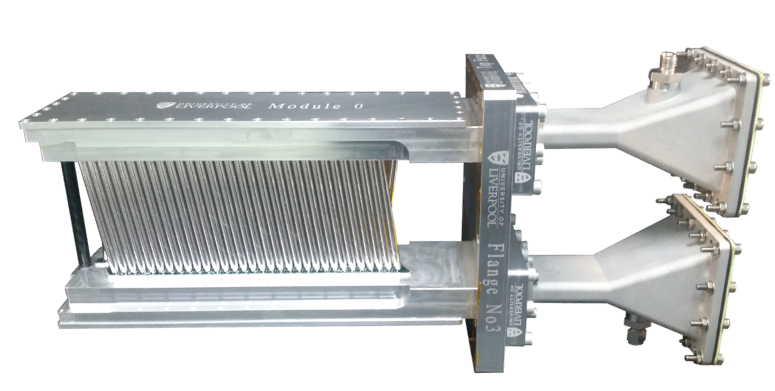
\includegraphics[trim={0 0 0 0},clip,width=.69\textwidth]{Images/Chapter3/TrackerModule.png}\label{subfig:TrackerModule}}
\hfill
\subfloat[]{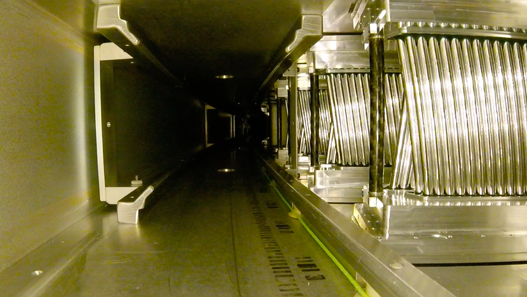
\includegraphics[trim={0 0 0 0},clip,width=.69\textwidth]{Images/Chapter3/Tracker-InVac.png}\label{subfig:TrackerInVac}}
\caption{Photographs of the straw trackers, showing: (a) an individual module, with two of the four layers Mylar straws visible; (b) a photograph taken from the interior of the vacuum chamber, showing a tracker station from the perspective of the muon beam. Images courtesy of the E989 collaboration.}
\label{fig:TrackerPhotos}
\end{figure} 

There are two tracker stations, referred to as stations 12 and 18\footnote{Named after the numbering of the extruded vacuum chamber sections shown in Figure \ref{fig:RingSchematic}, counting from zero.} in this thesis (indicated by T1 and T2 in Figure \ref{fig:RingSchematic}), positioned at approximately $180\degree$ and $270\degree$ around the ring. Each station is composed of a row of eight modules which are inserted into the vacuum chamber. The individual modules consist of four layers of 32 Mylar tubes, called straws, which are fixed to aluminium manifolds. The straws are \SI{5}{\milli\metre} in diameter, \SI{10}{\centi\metre} in length, and have a wall thickness of \SI{15}{\micro\metre}. Each straw encloses an atmosphere of equal parts argon and ethane, at a pressure of 1 atm, at centre of which is a \SI{25}{\micro\metre} diameter gold-plated tungsten sense-wire held at a positive potential difference of \SI{1.65}{\kilo\volt}. The sense-wire acts as an anode and the electrically grounded straw walls acts as a cathode, resulting in a strong radial electric field around the wire. When a positron traverses the interior of a straw it creates a trail of primary ionisation products (electrons and positive ions) in its wake. Compelled by the electric field, the electrons drift towards the wire, creating an avalanche of secondary ionisation products in the process, and cause an accumulation of charge on the wire which is registered as a hit. Meanwhile, the positive ionisation products are neutralised by the straw walls. Straw layers are alternately orientated at $\pm7.5\degree$ from the vertical, labelled U and V layers, enabling the vertical component of positron trajectory to be measured. The components of the trackers are constructed from non-magnetic materials so as not to perturb the magnetic field, and extensive leak testing was carried out to ensure that the tracker gas does not disturb the storage region vacuum \cite{Charity}. Photographs of the tracker modules are shown in Figure \ref{fig:TrackerPhotos}, and a rendering of the arrangement of modules relative to the vacuum chamber, and downstream calorimeter, can be found in Figure \ref{fig:TrackerSchematic}. Further discussion on the tracker design and performance can be found in \cite{Tracker}.

% \begin{figure}[t!]
% \centering{}
% 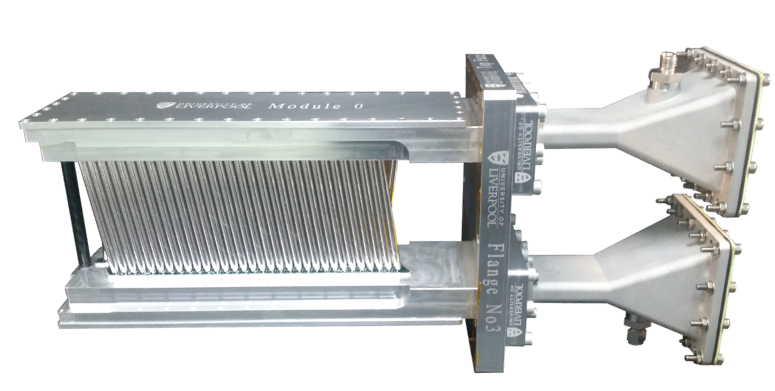
\includegraphics[trim={0 0 0 0},clip,width=.89\textwidth]{Images/Chapter3/TrackerModule.png}
% \caption{A photograph of an individual module: four layers of 32 Mylar straws, each containing a high voltage sense wire in a two of the four layers Mylar straws visible. Image courtesy of the E989 collaboration.}
% \label{fig:TrackerModule}
% \end{figure}

Tracks as formed by first grouping straw hits into \SI{80}{\nano\second} windows, which is less than the maximum drift time within a straw, to create `time islands'. Within the time island, hits are clustered by UV layer into singlets and doublets, e.g., if there are hits in both layers then the cluster is a doublet. Neighbouring clusters are then grouped together to form `track candidates'. Next, the correlation between drift times in adjacent layers is used to calculate an initial time, $t_{0}$, from which the drift times of individual hits are calculated. Using a calibrated relationship between drift time and distance, the `distance of closest approach' (DCA) of a positron to the sense wire is then calculated for each hit. Track fitting is then performed on candidates using a \texttt{GEANE} (Geometry and Error Propagation) \cite{GEANE} based $\chi^{2}$ minimisation algorithm developed by N. Kinnaird \cite{Kinnaird}. 

In order to characterise positron parameters at the muon decay point, such as the decay angle, tracks are extrapolated backwards, through a region of varying magnetic field, using method developed by S. Charity \cite{Charity}. This method relies on a Runge-Kutta-Nyström algorithm \cite{Runge} to find the point of radial tangency, or the point where the radial component of momentum is zero, which is considered to be a reliable estimate of the decay point. The resolution of track extrapolated parameters is discussed, in the context of the muon EDM search, in Chapter \ref{chap:6} Section \ref{subsec:TrackResolution}.

Finally, cuts are imposed on the parameters of tracks and extrapolated vertices in order to obtain a sample of what are referred to in this thesis as `quality tracks', or `quality vertices'. An example of a track-level quality requirement is that the track fit has a p-value of $>0.05$, and an example of a vertex-level quality requirement is that the positron does not scatter through a large volume of material before detection \cite{TrackQuality}.

\section{Measurement periods}\label{sec:MeasPeriods}

At the time of writing, E989 is nearing the end of its fifth data-taking period, called `Run-5'. The work presented in this thesis is primarily focused on an analysis of Run-1 data, supported by radial magnetic field measurements carried out in Run-4 (described in Chapter \ref{chap:4}). Run-6, which may involve running with $\mu^{-}$ as opposed to $\mu^{+}$, is likely to take place in 2022/2023. The total number of measured positrons over time is expressed in terms of the fraction of the BNL E821 cumulative dataset in Figure \ref{fig:ctag}, where the E989 raw integrated dataset is presently a factor of $\sim$18 times larger than that of E821. 

Run-1 is divided into four datasets, labelled `1a' through to `1d'. The statistical precision of the muon EDM search presented in Chapter \ref{chap:6} is governed by the numbers of quality-cut-passing tracks and extrapolated track decay vertices per Run-1 dataset, which are summarised in Table \ref{tbl:MeasPeriods}. Also included are the ESQ field indices, and corresponding voltages, which are relevant to the radial magnetic field analysis detailed in Chapter \ref{chap:4}. 

\begin{figure}[t!]
\centering{}
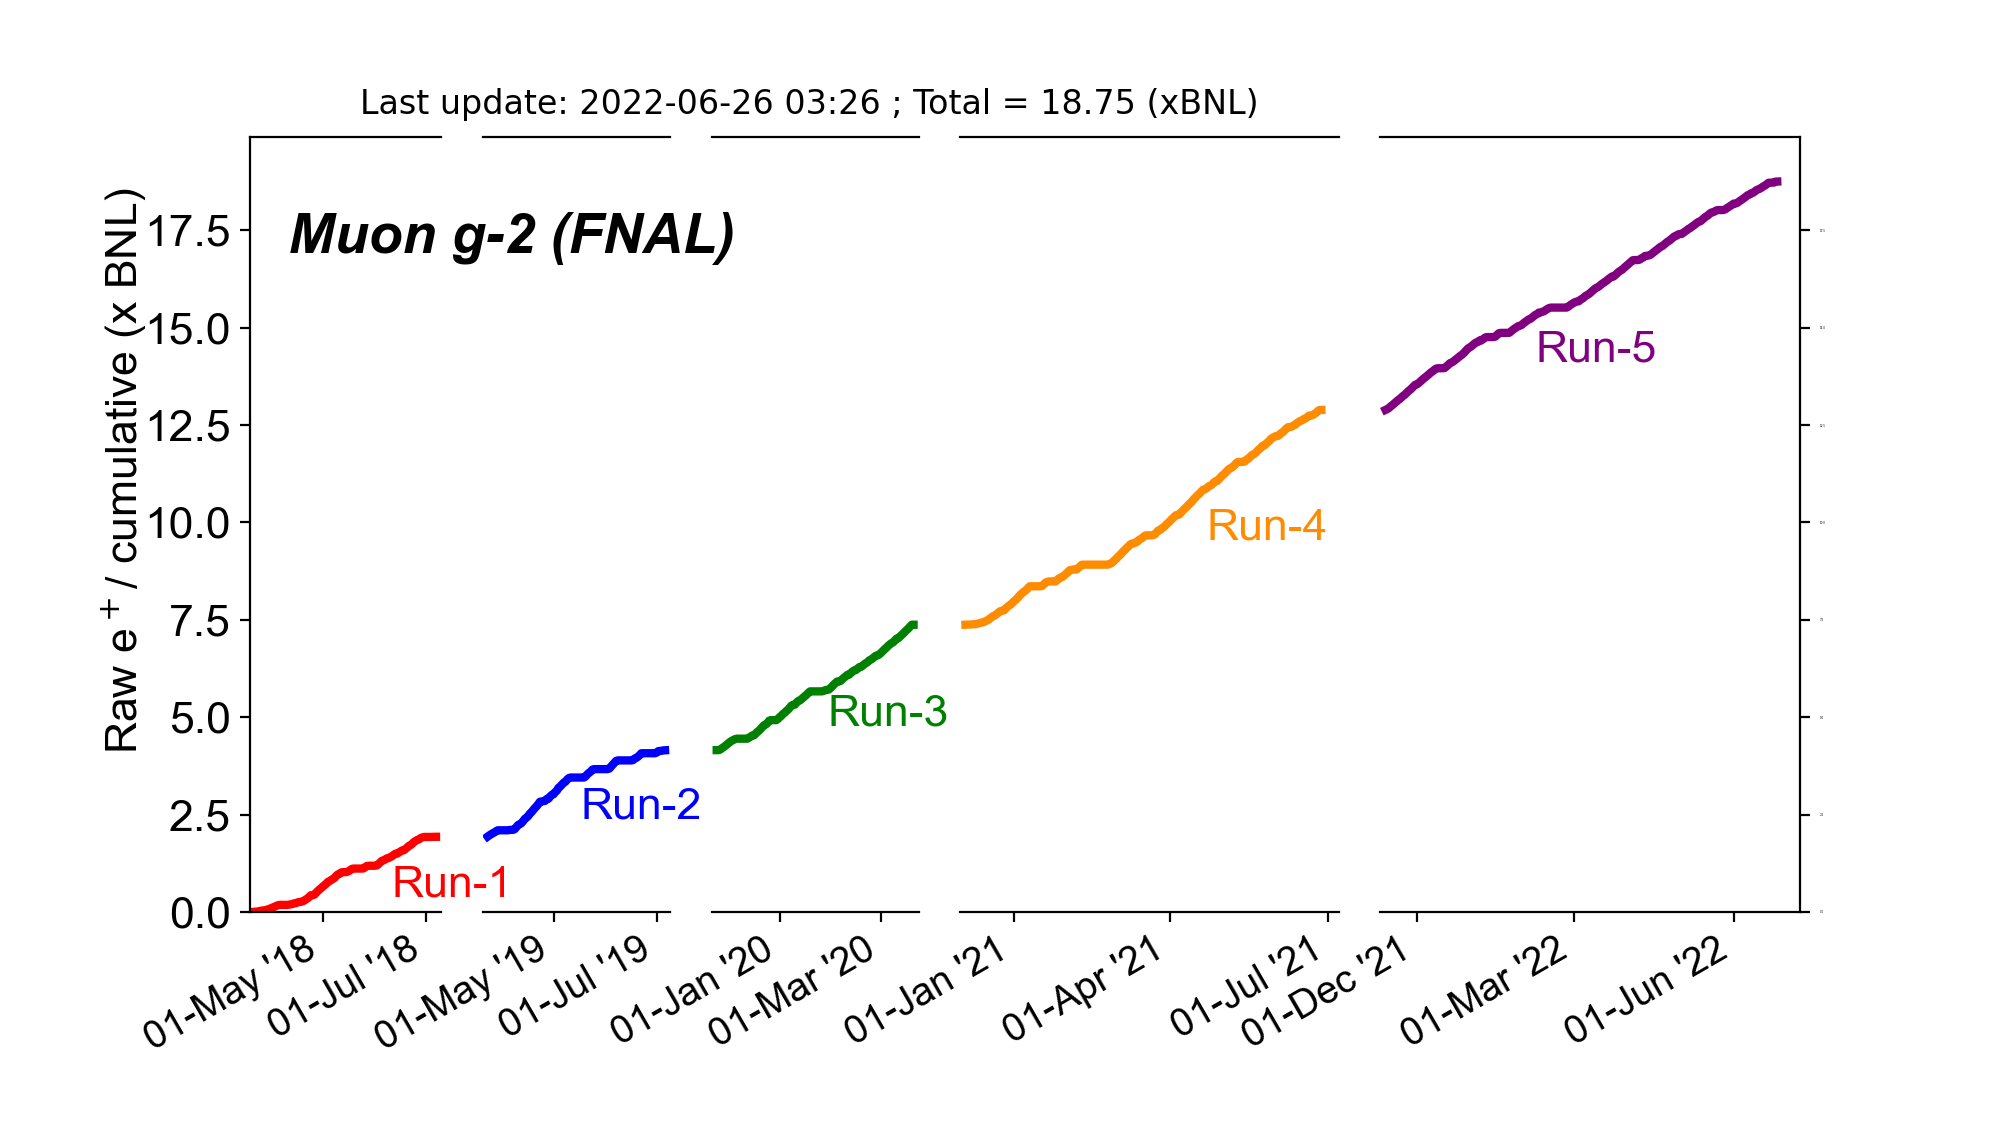
\includegraphics[trim={0 0 0 1.5cm},clip,width=\textwidth]{Images/Chapter3/integratedctag.png}
\caption{The raw integrated E989 dataset at the time of writing, expressed as fraction of the BNL E821 cumulative dataset. Image courtesy of M. Lancaster.}
\label{fig:ctag}
\end{figure}

\begin{table}[t!]
\centering
\begin{tabular}{l|cccc}
\hline
\hline
Dataset & Quality tracks & Quality vertices & ESQ field index, $n$ & ESQ voltage [kV] \\
\hline
Run-1a & $3.54\times10^{7}$ & $1.81\times10^{7}$ & 0.108 & 18.3 \\ 
Run-1b & $4.86\times10^{7}$ & $2.49\times10^{7}$ & 0.120 & 20.4 \\
Run-1c & $7.28\times10^{7}$ & $3.71\times10^{7}$ & 0.120 & 20.4 \\
Run-1d & $1.41\times10^{8}$ & $7.22\times10^{7}$ & 0.108 & 18.3 \\
\hdashline
Total & $2.98\times10^{8}$ & $1.52\times10^{8}$ & -- & -- \\ 
\hline
\hline
\end{tabular}
\caption{The numbers of high quality tracks and extrapolated track vertices for each Run-1 dataset, along with the ESQ field indices and corresponding voltages.}
\label{tbl:MeasPeriods}
\end{table}

\section{Overview of computing}\label{sec:Computing}

\begin{figure}[t!]
\centering{}
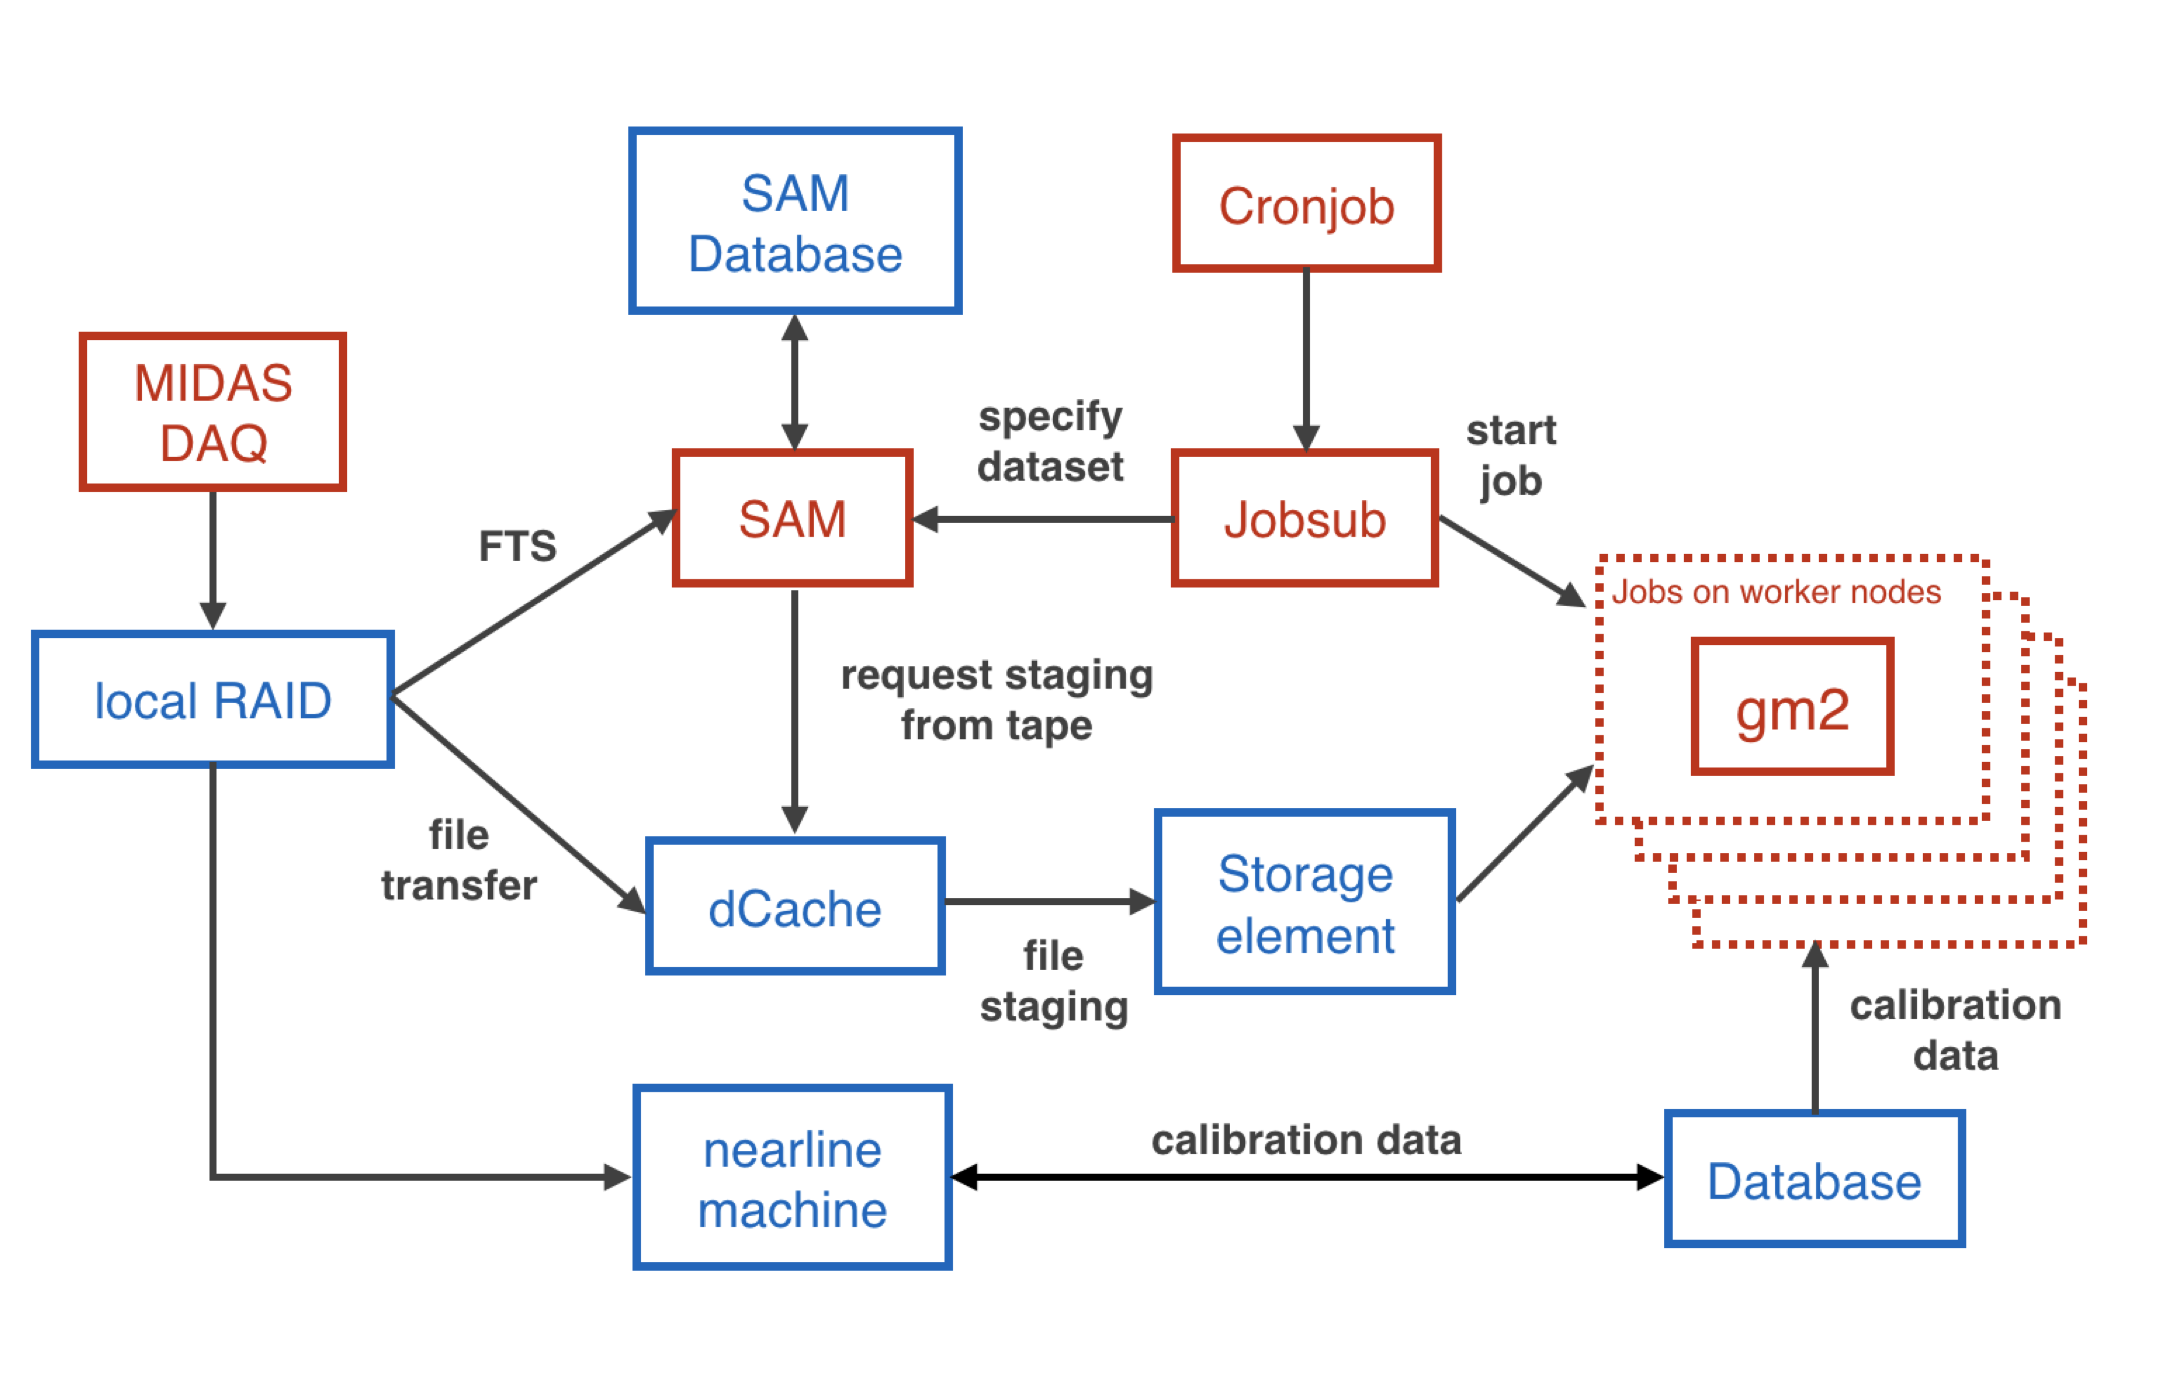
\includegraphics[trim={0 0 0 0},clip,width=.85\textwidth]{Images/Chapter3/DataRecoFlowDiagram.png}
\caption{A diagram illustrating the flow of data at E989, from the acquisition of raw data to high level analysis. Image reproduced from \cite{DataReco}.}
\label{fig:DataRecoFlow}
\end{figure}

The computing framework at E989 is split between an online data acquisition (DAQ), and offline data processing and simulation. The \texttt{MIDAS} \cite{MIDAS} based DAQ system handles the exceptionally high rate of raw data produced by the experiment while receiving beam ($\sim$20 GB/s) -- predominantly from 1296 calorimeter channels (54 channels per calorimeter). After receiving triggers from the accelerator complex, the DAQ system processes the raw calorimeter data into `derived datasets' (such as islands of digitized pules) with 28 NVIDIA \textit{K40} GPUs working in parallel, writing binary files in \texttt{MIDAS} format to temporary storage on local RAID array, after which they are transferred to tape for permanent on-site storage using the \texttt{dCache} system at a much reduced rate of $\sim$200 MB/s. The experiment also utilises a data quality monitor (DQM), which reconstructs a subset of the data, providing live feedback as to the status of the experiment during operation. In addition, high level \texttt{ROOT} \cite{ROOT} histograms and \texttt{Ntuples} are produced on a multi-core nearline (NL) machine, writing output to a local disk which may be accessed by users via a web server. Once written to tape, the data is fully reconstructed and organised into datasets using the sequential access via metadata (SAM) \cite{SAM} cataloguing service. This in an automated procedure called `data production', which relies heavily on grid computing: a combination of FermiGrid \cite{FermiGrid} and Open Science Grid \cite{OSG}. For simulation, E989 employs a \texttt{GEANT4} \cite{GEANT4} based model of the storage ring and detector systems called \texttt{gm2ringsim}. Event processing, both for data and simulation, is handled by use of Fermilab's \texttt{C++} based \texttt{art} framework \cite{art}. A diagram illustrating the flow of data in at E989 is given in Figure \ref{fig:DataRecoFlow}. Further information on E989 computing can be found in \cite{KimSiangComputing}.


\afterpage{
\begin{figure}[]
\centering{}
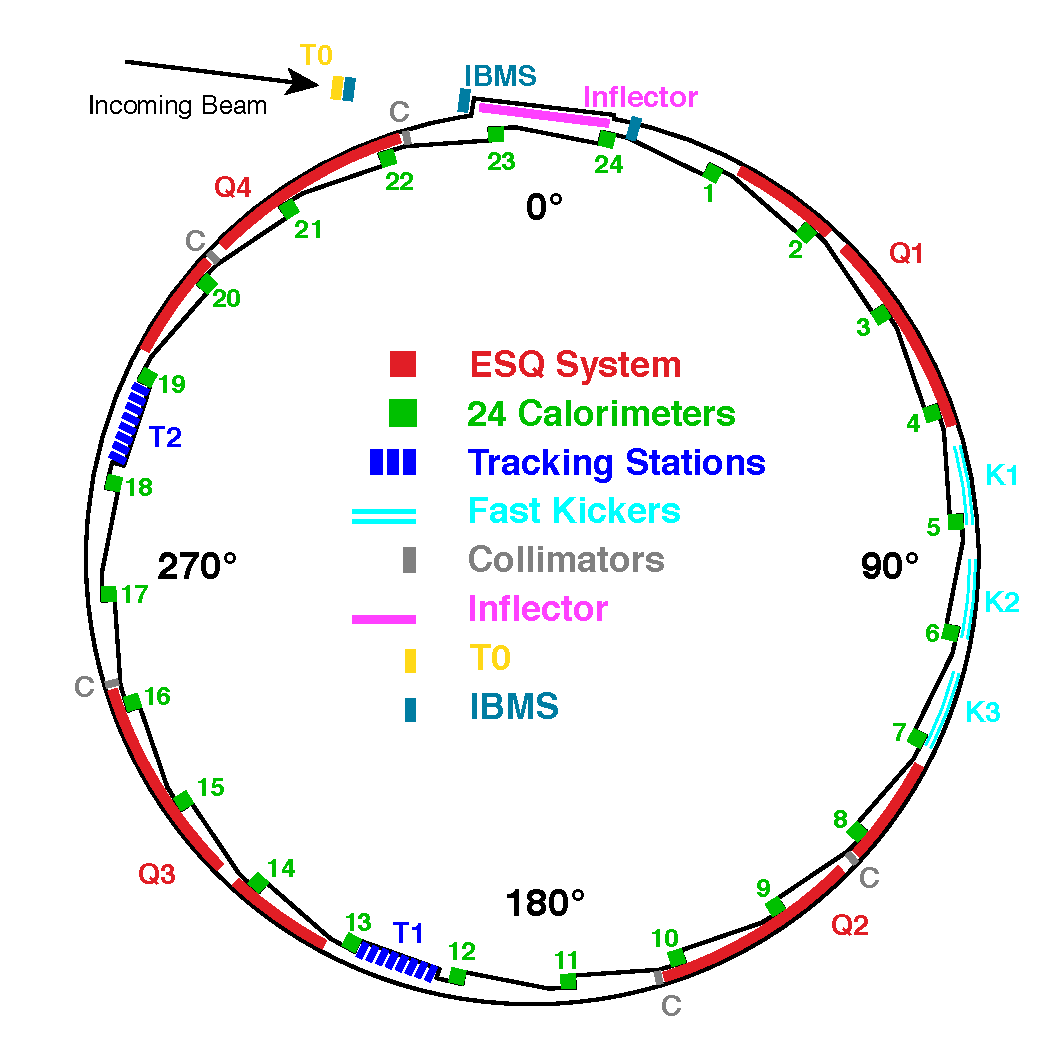
\includegraphics[trim={0 0 0 0},clip,width=\textwidth]{Images/Chapter3/RingSchematic.pdf}
\caption{A schematic of the E989 storage ring, illustrating the various components discussed in this chapter. Image reproduced from \cite{BeamDynamics}.}
\label{fig:RingSchematic}
\end{figure}
\clearpage
}